% Last Update: $Id$


\include{fli4l}
\makeindex

\begin{document}

\newcommand{\titlename}{Paket OPENVPN}

\flhypersetup{pdftitle=\titlename}
\pdfbkmrk{-1}{\titlename}{title}
\title{\titlename\\ Version \version}

\author{Claas Hilbrecht\\ \email{babel (+at+) fli4l dot de} \and Das fli4l-Team\\ \email{team@fli4l.de}}

\maketitle
\pdfbkmrk{0}{\contentsname}{table}
\tableofcontents

\chapter{Dokumentation des Paketes OPENVPN}

% Do not remove the next line
% Synchronized to r49522

\marklabel{sec:openvpn}{
  \section{OpenVPN~- Supporte le VPN}}
\hyphenation{OpenVPN}

\sloppy

Depuis la version 2.1.5, le paquetage OpenVPN fait partie intégrante de fli4l.

\wichtig{Avec l'utilisation du paquetage VPN vous pouvez installer un tunnel VPN
sur Internet, il est nécessaire d'avoir soit, un forfait d'accès Internet illimité
soit un forfait avec un volume heure important~! Le routeur fli4l reste allumé en
permanence, la connexion ne peut pas être coupée, étant donné que les données sont
transférées en permanence sur le tunnel (même si c'est quelques octets pendant quelques
secondes), les frais de communications seront élevés si vous utilisez un forfait avec
un volume d'heures liminés, il en va de même si vous choisissez une connexion ISDN.}

Il y a dans la base de données OPT sur le site \altlink{http://www.fli4l.de/fr/telechargement/paquetage-annexe/},
en plus du tunnel OpenVPN le paquetage OPT\_PoPToP pour la création de tunnel.

Le fait d'opter pour une solution VPN, dépend en premier lieu de la sécurité et des
fonctionnalités l'installation. Voici Des rapports sur la sécurité et des solutions
pour des réseaux privés virtuels, l'équipe fli4l n'est pas concerné sur ces rapport,
voici des pages Web sur ces rapports~:

Magazin Linux numéro janvier 2004

\altlink{http://diswww.mit.edu/bloom-picayune/crypto/14238}

\altlink{http://sites.inka.de/bigred/archive/cipe-l/2003-09/msg00263.html}

%\altlink{http://groups.google.de/groups?dq=&hl=de&lr=&ie=UTF-8&oe=UTF-8&th=5dd52cd0d5592e5d&seekm=blsm3q%24lhk%2403%241%40news.t-online.com#link1}

%\altlink{http://www.linuxsecurity.com/feature_stories/feature_story-152.html}

L'équipe fli4l a une position claire sur la fonctionnalité d'OpenVPN. Sur ce point,
OpenVPN est le gagnant, le meilleur par rapport à Poptop. OpenVPN supporte
avec le tunnel le module Bridge et une compression des données, contrairement à Poptop,
en plus il est stable sur le routeur fli4l. il existe également une version OpenVPN
pour Windows, qui peut être utilisé à partir de Windows 2000. Les seuls inconvénients
d'OpenVPN par rapport à Poptop est la taille de l'archive opt et la version
2.0.x de fli4l qui n'est pas supportée par OpenVPN.


\subsection{OpenVPN~- Introduction et exemple}

Pour entrer plus facilement dans la configuration, vous pouvez voir dans l'exemple
ci-dessous. Deux réseaux qui utilise chacun un routeur fli4l connecté à Internet.
Avec l'installation d'OpenVPN (tunnel codé) sur les routeurs fli4l, les ordinateurs
des deux réseaux pourront communiquer entre eux par Internet dans des villes différentes.
Et aussi les variables de configuration dans la figure \ref{fig:tunnel}.

  \begin{figure}[htbp]
    \centering
    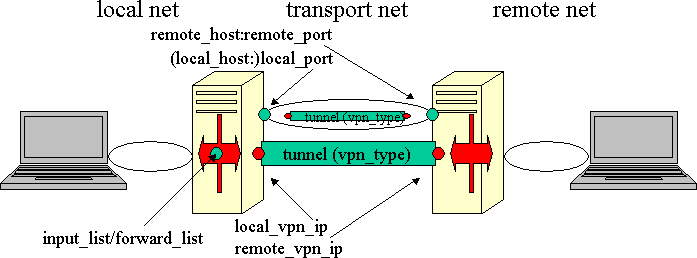
\includegraphics[width=\columnwidth]{openvpn-sample}
    \caption{Exemple de configuration VPN --- Tunnel entre deux routeurs}
    \label{fig:tunnel}
  \end{figure}

  \begin{description}

  \item [local net, remote net] La figure représente deux réseaux reliés entre eux par un
  tunnel. Les deux réseaux reliés doivent avoir un TCP/IP différent et ne doivent pas non plus
  s'entrecroiser avec leurs masques de sous-réseau. Le réglage respectif \jump{IPNETx}{\var{IP\_NET\_x}}
  dans le fichier de configuration base.txt ne doivent pas être le même que le
  tunnel VPN. Si les deux réseaux utilisent la même adresse IP 192.168.6.0/24
  ils ne peuvent pas être liés par un tunnel VPN.

  \item [transport net] Le réseau de transport se compose de deux éléments~:

  \begin{itemize}

  \item La connexion entre les deux démons OpenVPN, sont décritent dans
  \emph{\smalljump{OPENVPNxREMOTEHOST}{remote\_host}~: \smalljump{OPENVPNxREMOTEPORT}{remote\_port}} et
  \emph{\smalljump{OPENVPNxLOCALHOST}{local\_host}~: \smalljump{OPENVPNxLOCALPORT}{local\_port}}.
  Cela correspond aux paramètres de configuration OpenVPN~: \var{OPENVPN\_x\_REMOTE\_HOST},
  \var{OPENVPN\_x\_REMOTE\_PORT}, \var{OPENVPN\_x\_LOCAL\_HOST} et
  \var{OPENVPN\_x\_LOCAL\_PORT}.

  \item Le tunnel, sur lequel la liaison entre les démons OpenVPN est établie, sont décritent dans
  \emph{\smalljump{OPENVPNxLOCALVPNIP}{local\_vpn\_ip}/\smalljump{OPENVPNxREMOTEVPNIP}{remote\_vpn\_ip}}.
  Cela correspond alors à~: \var{OPENVPN\_x\_LOCAL\_VPN\_IP} et \var{OPENVPN\_x\_REMOTE\_VPN\_IP}.
  Les deux adresses IP sont uniquement utilisé pour le VPN et se trouvent dans les deux
  routeurs du réseau connus.

  \end{itemize}

  \item Les variables [\smalljump{OPENVPNxPFINPUTN}{input\_list} et \smalljump{OPENVPNxPFFORWARDN}{forward\_list}]
  servent à filtrer les paquets qui circulent dans le tunnel. Le seule filtre
  autorisé que l'on peut utiliser et qui permet à tester le tunnel par des messages
  standards est ICMP (exemple le ping). Dans tout les autres cas, on doit
  d'abord autoriser les paquets explicitement, voici le cas le plus simple~:

\begin{example}
\begin{verbatim}
OPENVPN_x_PF_INPUT_POLICY='ACCEPT'
OPENVPN_x_PF_FORWARD_POLICY='ACCEPT'
\end{verbatim}
\end{example}

  \achtung{N'oubliez pas que si vous \flqq{}ouvrez\frqq{} complètement les liaisons
  VPN, cela pourrais être dangereux pour la sécurité. Utilisez plutôt le tmpl: fichier
  de syntaxe pour le filtrage de paquets, afin d'ouvrir uniquement les services que vous
  avez besoin.}

  \end{description}

  Il n'est pas nécessaire de paramétrer d'avantage de variables pour un simple tunnel VPN.
  Toutes les autres possibilités de réglage traitent des fonctionnalités avancées, ils sont
  disponibles pour des applications spéciales. Avec un minimum de réglage le tunnel VPN
  peut fonctionner, si vous paramétrez les variables avancées celles-ci doivent d'être
  compatibles pour un bon fonctionnement.


\subsection{OpenVPN~- Configuration}

  Puisqu'OpenVPN est assez complexe, nous commencerons par les variables obligatoires,
  nécessaires pour une liaison VPN. Ce n'est que lorsque le routeur fli4l sera connecté
  avec ces paramètres, que vous pourrez vous lancer à configurer les autres variables pour
  une utilisation étendues d'OpenVPN.

\begin{description}

\config{OPT\_OPENVPN}{OPT\_OPENVPN}{OPTOPENVPN}

  Par défaut~: \var{OPT\_OPENVPN='no'}

  Avec \var{'yes'} vous activez le paquetage OpenVPN. Avec \var{'no'} vous désactivez
  complétement le paquetage OpenVPN.

\config{OPENVPN\_N}{OPENVPN\_N}{OPENVPNN}

  Par défaut~: \var{OPENVPN\_N='0'}

  Dans cette variable vous indiquez le nombre de configuration OpenVPN à activer.

\config{OPENVPN\_x\_REMOTE\_HOST}{OPENVPN\_x\_REMOTE\_HOST}{OPENVPNxREMOTEHOST}

  Par défaut~: \var{OPENVPN\_x\_REMOTE\_HOST=''}

  Vous indiquez ici l'adresse IP ou l'adresse DNS du poste OpenVPN distant. Dans le
  cas d'un \jump{roadwarrior}{Roadwarrior} (on peut dire "commerciaux nomade
  informatisés") vous devez laisser cette variable vide. Si le paramètre est omis,
  OpenVPN attendra une connexion, il ne tentera pas de se connexion.

\config{OPENVPN\_x\_REMOTE\_HOST\_N}{OPENVPN\_x\_REMOTE\_HOST\_N}{OPENVPNxREMOTEHOSTN}

  Par défaut~: \var{OPENVPN\_x\_REMOTE\_HOST\_N='0'}

  Lorsque l'on utilise un service DNS dynamique, ce service n'est malheureusement pas fiable
  à 100\%. C'est pourquoi il est plus simple dans n'installer deux, voire plusieurs services
  DynDNS différent et d'enregistrer en même temps une seul adresse IP pour tous ces services.
  Ainsi OpenVPN vérifira tout les noms DynDNS, dans cette variable on enregistre le nombre
  de nom de DNS \emph{supplémentaire}. dans la variable \var{OPENVPN\_x\_REMOTE\_HOST}
  on enregistrera la liste des adresses, OpenVPN essaira de contacter cette liste dans un
  ordre aléatoire. La variable \var{OPENVPN\_x\_REMOTE\_HOST} doit donc continuer d'exister~!

\config{OPENVPN\_x\_REMOTE\_HOST\_x}{OPENVPN\_x\_REMOTE\_HOST\_x}{OPENVPNxREMOTEHOSTx}

  Par défaut~: \var{OPENVPN\_x\_REMOTE\_HOST\_x=''}

  Il s'agit de la même description que la variable \jump{OPENVPNxREMOTEHOST}{\var{OPENVPN\_x\_REMOTE\_HOST}}
  on place ici l'adresse DynDNS ou l'adresse IP statique.

\config{OPENVPN\_x\_REMOTE\_PORT}{OPENVPN\_x\_REMOTE\_PORT}{OPENVPNxREMOTEPORT}

  Par défaut~: \var{OPENVPN\_x\_REMOTE\_PORT=''}

  Lorsque OpenVPN est connecté, on a besoin sur le routeur fli4l un Port qui n'est pas
  encore utilisé. Il est recommandé d'utiliser les ports au delà de 10000, car ces ports
  ne sont généralement pas utilisés. Lorsque vous voulez déployer une liaison vers un
  poste distant, si ce poste a une adresse IP dynamique et s'il n'a pas d'adresse DynDNS,
  vous pouvez laisser cette variable vide exactement comme la variable \var{OPENVPN\_x\_REMOTE\_HOST}.

\config{OPENVPN\_x\_LOCAL\_HOST}{OPENVPN\_x\_LOCAL\_HOST}{OPENVPNxLOCALHOST}

  Par défaut~: \var{OPENVPN\_x\_LOCAL\_HOST=''}

  On indique ici l'adresse IP qui doit être connecté à l'OpenVPN. Cette entrée doit
  rester vide ou complètement omise lors de connexion Internet. Si une adresse IP est
  indiqué ici, OpenVPN écoute les demandes de connexion entrante uniquement sur cet
  adresse IP. Si vous voulez assurer une connexion WLAN, vous devez enregistrer ici
  l'adresse IP de la carte WLAN qui est sur le routeur fli4l.

\config{OPENVPN\_x\_LOCAL\_PORT}{OPENVPN\_x\_LOCAL\_PORT}{OPENVPNxLOCALPORT}

  Par défaut~: \var{OPENVPN\_x\_LOCAL\_PORT=''}

  On indique ici le numéro du Port, sur lequel le démon OpenVPN écoute. Pour chaque
  configuration d'OpenVPN vous aurez besoin de réserver le port, c.-à-d. que ce port ne
  peut être utilisé que par la liaison OpenVPN et ne peut être utilisé par aucun autre
  programme sur le routeur fli4l. Les paramètres des variables 
  \var{OPENVPN\_x\_REMOTE\_PORT} et \var{OPENVPN\_x\_LOCAL\_PORT} doivent être installé
  pour une liaison OpenVPN~! Si vous paramétrez la variable \var{OPENVPN\_x\_REMOTE\_PORT='10111'}
  d'un côté du tunnel, on \emph{doit} impérativement placer de l'autre côté du tunnel
  dans la variable \var{OPENVPN\_x\_LOCAL\_PORT='10111'} le même port.

  Encore une fois~: il est très important d'ajuster ces réglages sur les deux côtés respectifs
  de l'OpenVPN, autrement la liaison entre les partenaires OpenVPN ne sera pas possible.

  Afin qu'OpenVPN puisse écouter les connexions entrantes, OpenVPN ouvre indépendamment
  les ports qui sont indiqués dans la variable \var{OPENVPN\_x\_LOCAL\_PORT} pour le
  filtrage de paquets. Si vous ne le souhaité pas, vous pouvez ajuster les ports dans
  la variable \jump{OPENVPNDEFAULTOPENOVPNPORT}{\var{OPENVPN\_DEFAULT\_OPEN\_OVPNPORT}}.
  Il n'est pas nécessaire d'activer la variable \var{OPENVPN\_DEFAULT\_OPEN\_OVPNPORT='yes'}
  puisque c'est le paramètre par défaut~!

  Il n'est pas possible pour OpenVPN d'écouter des ports en dessous de 1025. Si vous voulez
  configurer un port en dessous comme par ex. si vous voulez configurer OpenVPN comme
  serveur tcp4 ou tcp6 sur le port 443 (port https), vous devez transmettre par le port 443 les
  paquets filtrés vers un port supérieur à 1024. Par ex votre OpenVPN écoute sur le port
  5555 il transmettra les paquets vers le port 443, cela doit être enregistré dans la
  variable \var{PF\_PREROUTING} comme ceci.

\begin{example}
\begin{verbatim}
PF_PREROUTING_5='tmpl:https dynamic REDIRECT:5555'
\end{verbatim}
\end{example}

\config{OPENVPN\_x\_SECRET}{OPENVPN\_x\_SECRET}{OPENVPNxSECRET}

  Par défaut~: \var{OPENVPN\_x\_SECRET=''}

  OpenVPN a besoin pour crypter une connexion OpenVPN d'un soi-disant fichier clé.
  Ce fichier clé peut être produit directement avec OpenVPN sous Windows ou Linux.
  Pour les débutants, vous avez soit le logiciel OpenVPN sous Windows ou soit le
  WebGUI, interface graphique pour OpenVPN. Si vous ne voulez pas utiliser OpenVPN
  sous Windows, mais créer seulement le ou les fichiers clés pour OpenVPN, il suffit,
  d'installer ces quelques fichiers \emph{OpenVPN User-Space Components}, \emph{OpenSSL DDLs},
  \emph{OpenSSL Utilities}, \emph{Add OpenVPN to PATH} et \emph{Add Shortcuts to OpenVPN}.
  Au démarrage d'OpenVPN vous avez dans le menu la commande \emph{Generate a static OpenVPN key},
  qui est nécessaire pour produire le fichier clé. Après avoir activé cette commande
  dans le menu, un message apparais \flqq{}Randomly generated 2048 bit key written to
  \var{C:/Programme/OpenVPN/config/key.txt}\frqq{}. Le fichier \var{key.txt} sera
  créé il est essenciel pour l'utilisation de ce fichier, de copier celui-ci dans
  le répertoire \var{$<$config$>$/etc/openvpn} et de renommer le fichier \var{key.txt}
  de façon à ce que le nom du fichier soit significatif pour être placé dans cette variable.\\
  Vous pouvez aussi produire le fichier clé automatiquement au démarrage du routeur fli4l,
  pour cela, vous devez mettre la variable \var{OPENVPN\_CREATE\_SECRET} sur
  \var{'yes'}. Si vous configurez pour la première fois OpenVPN, vous devez
  enregistrer toutes les données du fichier config et placer la variable
  \jump{OPENVPNDEFAULTCREATESECRET}{\var{OPENVPN\_DEFAULT\_CREATE\_SECRET}} sur \var{'yes'},
  vous pouvez produire plusieurs fichiers clés pour plusieurs liaisons OpenVPN ou
  produire qu'un seul fichier clé pour une liaison OpenVPN, pour cela vous devez
  placer la variable \var{OPENVPN\_x\_CREATE\_SECRET} sur \var{'yes'}. Après le
  démarrage du routeur fli4l, le ou les fichiers clé(s) seront alors produits
  automatiquement et placés ces fichiers dans le dossier \var{/etc/openvpn} avec
  leur nom respectif, voir ci-dessous. Le ou les fichiers clé(s) peuvent alors
  être transféré avec le SCP ou copié sur le support de boot. Vous devez replacer
  la variable de création de fichier clé sur 'no'. Ne laissez pas la variable de
  création de clé sur 'yes' car à chaque redémarrage du routeur fli4l de nouveaux
  fichiers clés seront produits par le démon OpenVPN. Il sera alors impossible de
  déployer le tunnel VPN.\\
  Si vous voulez utiliser l'interface Web pour produire le ou les fichiers clé(s),
  vous devez mettre la variable \var{OPENVPN\_x\_CREATE\_SECRET} sur \var{'webgui'}.
  Vous devez vous connecter sur l'interface Web, dans la fenêtre générale
  sélectionner gestion clé. Pour plus de précision vous pouvez aller voir
  le paragraphe \ref{sec:openvpn_gui}.

  Astuce~: avec la commande
  \begin{verbatim}
      openvpn --genkey --secret <dateiname>
  \end{verbatim}
  vous pouvez produire par ligne de command un fichier clé sur la console du routeur fli4l.

  Les fichiers clés doivent être copiés dans le dossier \var{$<$config$>$/etc/openvpn}
  comme indiqué dans l'illustration ci-dessous. Le nom du ou des fichiers clés doivent
  ensuite être placé dans la variable \var{OPENVPN\_x\_SECRET}. Alors, les fichiers
  clés seront compactés et intégrés dans le fichier opt-Archives.

  \begin{figure}[htbp]
    \centering
    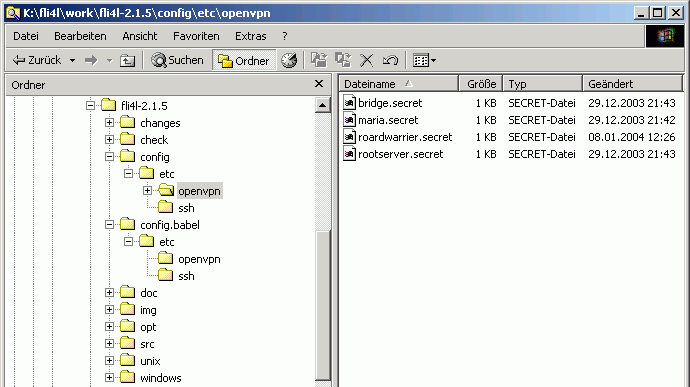
\includegraphics[width=\columnwidth]{config_etc_openvpn}
    \caption{fli4l répertoire OpenVPN avec les fichiers *.secret}
    \label{fig:config_etc_openvpn}
  \end{figure}

\config{OPENVPN\_x\_TYPE}{OPENVPN\_x\_TYPE}{OPENVPNxTYPE}

  Par défaut~: \var{OPENVPN\_x\_TYPE=''}

  On peut utiliser une liaison OpenVPN soit par tunnel, soit par Bridge. OpenVPN
  par tunnel utilise exclusivement le trafic IP routé. OpenVPN par bridge, le
  transfère se fait non seulement en trafic IP et aussi en frames Ethernet,
  par ex. avec le protocole IPX ou NetBEUI. Si vous utilisez OpenVPN avec le
  transport frames Ethernet, dans tous les cas le paquetage advanced\_networking
  est nécessaire. Veuillez considérer que l'utilisation du Bridging avec une
  connexion DSL peut être lente~!

\end{description}


\subsection{OpenVPN~- Configuration du bridge}

  Si vous utilisez OpenVPN avec Bridge, vous pouvez paramétrer les entrées
  suivantes, N'oubliez pas, que lors de l'utilisation d'un Bridge sur Internet,
  avec le trafic Broadcast on a besoin d'une bande passante relativement élevée.

  Considérer que les réglages suivants ne sont valables que si la variable
  \jump{OPENVPNxTYPE}{\var{OPENVPN\_x\_TYPE}} a été paramétrée sur \var{'bridge'}
  pour une liaison OpenVPN~! En outre, la configuration du bridge dans le
  paquetage advanced\_networking est nécessaire, auquel cas la liaison VPN
  se bloque.

\begin{description}

\config{OPENVPN\_x\_BRIDGE}{OPENVPN\_x\_BRIDGE}{OPENVPNxBRIDGE}

  Par défaut~: \var{OPENVPN\_x\_BRIDGE=''}

  On indique ici, le nom du Bridge, avec lequel la liaison OpenVPN doit se faire.
  Donc si dans la variable \var{BRIDGE\_DEV\_x\_NAME='cuj-br'} du paquetage
  advanced\_networking le nom est \var{'cuj-br'}, vous devez indiquer
  également le même nom ici pour avoir une liaison OpenVPN par Bridge valide.

\config{OPENVPN\_x\_BRIDGE\_COST}{OPENVPN\_x\_BRIDGE\_COST}{OPENVPNxBRIDGECOST}

  Par défaut~: \var{OPENVPN\_x\_BRIDGE\_COST=''}

  Si vous utilisez STP (voir \altlink{http://de.wikipedia.org/wiki/Spanning_Tree}
  ou la documentation dans le paquetage advanced\_networking) vous pouvez
  indiquer ici le coût de la connexion.

\config{OPENVPN\_x\_BRIDGE\_PRIORITY}{OPENVPN\_x\_BRIDGE\_PRIORITY}{OPENVPNxBRIDGEPRIORITY}

  Par défaut~: \var{OPENVPN\_x\_BRIDGE\_PRIORITY=''}

  Si vous utilisez STP (voir \altlink{http://de.wikipedia.org/wiki/Spanning_Tree}
  ou la documentation dans le paquetage advanced\_networking) vous pouvez indiquer
  ici la priorité de la connexion.

\end{description}


\subsection{OpenVPN~- Configuration du tunnel}

\begin{description}

\config{OPENVPN\_x\_REMOTE\_VPN\_IP}{OPENVPN\_x\_REMOTE\_VPN\_IP}{OPENVPNxREMOTEVPNIP}

  Par défaut~: \var{OPENVPN\_x\_REMOTE\_VPN\_IP=''}

  Considérer que les réglages suivants ne sont valables que si la variable
  \jump{OPENVPNxTYPE}{\var{OPENVPN\_x\_TYPE}} a été paramétrée sur \var{'tunnel'}
  pour une liaison OpenVPN~!

  Adresse IP VPN du poste éloigné pour une liaison OpenVPN. Les adresses IP VPN
  sont nécessaires et peuvent être choisies presque librement. Ci-dessous les
  restrictions pour le choix d'une adresse IP VPN sont les suivantes~:

\begin{itemize}

\item L'adresse IP ne peut pas être utilisée dans le réseau local. Elle ne peut
  pas non plus se trouver dans le sous-réseau du routeur fli4l.

\item L'adresse IP ne peut pas être utilisé pour la restauration système par le réseau.

\item L'adresse IP ne peut pas faire partie d'un réseau \var{IP\_ROUTE\_x}.

\item L'adresse IP ne peut pas faire partie d'un réseau \var{ISDN\_CIRC\_ROUTE\_x}.

\item L'adresse IP ne peut pas faire partie d'un réseau \var{CIPE\_ROUTE\_x}.

\item L'adresse IP ne peut pas faire partie d'un réseau \var{OPENVPN\_ROUTE\_x}.

\item Il est entendu que l'adresse IP ne doit pas appartenir à un réseau fli4l
  ou à un réseau du routeur fli4l.

\end{itemize}

  Comme vous le voyez, l'adresse IP ne peut être utilisée nulle part ailleurs.
  Avant que vous commenciez la configuration d'OpenVPN, vous devez chercher une
  adresse IP qui n'est pas utilisée par de réseau, avec laquelle vous pouvez
  installer une liaison VPN. L'adresse IP du réseau devrait aussi absolument
  faire partie d'un réseau privé (voir \altlink{http://ftp.univie.ac.at/netinfo/rfc/rfc1597.txt}).

\config{OPENVPN\_x\_LOCAL\_VPN\_IP}{OPENVPN\_x\_LOCAL\_VPN\_IP}{OPENVPNxLOCALVPNIP}

  Par défaut~: \var{OPENVPN\_x\_LOCAL\_VPN\_IP=''}

  Ce réglage est valable, que si la variable \jump{OPENVPNxTYPE}{\var{OPENVPN\_x\_TYPE}}
  est paramétrée sur \var{'tunnel'} pour pouvoir régler une liaison OpenVPN.

  On indique ici l'adresse IP de l'OpenVPN local périphérique tunX. Le choix de
  l'adresse IP est soumis à la même restriction que la variable
  \jump{OPENVPNxREMOTEVPNIP}{\var{OPENVPN\_x\_REMOTE\_VPN\_IP}}.

  Il est d'ailleurs possible d'utiliser pour toutes les liaisons OpenVPN locale,
  la même adresse IP qui est dans la variable \var{OPENVPN\_x\_LOCAL\_VPN\_IP}.
  Ainsi, il est plus facilement pour un hôte utilisé la même adresse IP dans le
  VPN. Cela simplifie énormément les règles de filtrage de paquets.

\config{OPENVPN\_x\_IPV6}{OPENVPN\_x\_IPV6}{OPENVPNIPV6}

  Par défaut~: \var{OPENVPN\_x\_IPV6='no'}

  Avec cette variable vous pouvez activez le support IPv6 natif pour OpenVPN.
  Cette programmation est assez nouvelle et peut être qualifiée d'expérimentale.
  pour cela vous devez activer le paquetage OPT\_IPV6 et le configurer. Si vous
  indiquez \var{OPENVPN\_x\_IPV6='no'} et/ou \var{OPT\_IPV6='no'} ces variables
  sont en relations, elle sera ignorer.

  Attention~! Actuellement, il n'existe pas de contrôle si les informations se
  chevauchent avec d'autres parties de la configuration~! Ceci s'applique aux
  variables \var{OPENVPN\_x\_LOCAL\_VPN\_IPV6}, \var{OPENVPN\_x\_REMOTE\_VPN\_IPV6}
  et \var{OPENVPN\_x\_ROUTE\_x}.

\config{OPENVPN\_x\_REMOTE\_VPN\_IPV6}{OPENVPN\_x\_REMOTE\_VPN\_IPV6}{OPENVPNxREMOTEVPNIPV6}

  Par défaut~: \var{OPENVPN\_x\_REMOTE\_VPN\_IPV6=''}

  La variable IPv6 est égal à celle-ci \jump{OPENVPNxREMOTEVPNIP}{\var{OPENVPN\_x\_REMOTE\_VPN\_IP}}.

  \begin{example}
  \begin{verbatim}
    OPENVPN_X_REMOTE_IPV6='FD00::1'
  \end{verbatim}
  \end{example}

\config{OPENVPN\_x\_LOCAL\_VPN\_IPV6}{OPENVPN\_x\_LOCAL\_VPN\_IPV6}{OPENVPNxLOCALVPNIPV6}

  Par défaut~: \var{OPENVPN\_x\_LOCAL\_VPN\_IPV6=''}

  La variable IPv6 est la même que la variable \jump{OPENVPNxLOCALVPNIP}{\var{OPENVPN\_x\_LOCAL\_VPN\_IP}}.
  si vous n'indiquez pas de sous-réseau, /64 sera automatiquement utilisé comme
  sous-réseau.

  \begin{example}
  \begin{verbatim}
    OPENVPN_X_LOCAL_IPV6='FD00::2/112'
  \end{verbatim}
  \end{example}

\config{OPENVPN\_x\_ROUTE\_N}{OPENVPN\_x\_ROUTE\_N}{OPENVPNxROUTEN}

  Par défaut~: \var{OPENVPN\_x\_ROUTE\_N=''}

  Ce réglage n'est valable, que si la variable \jump{OPENVPNxTYPE}{\var{OPENVPN\_x\_TYPE}}
  est paramétrée sur \var{'tunnel'} pour pouvoir régler une liaison OpenVPN.

  Les routes (ou les destinations) données seront lu automatiquement, aussitôt
  qu'OpenVPN est démarré. On indique ici le nombre de route, on peut mettre
  jusqu'à 50 réseaux pour une liaison OpenVPN. Il faudra tout de même pour
  chaque réseau indiquer une adresse IP dans une variable différente
  \var{OPENVPN\_x\_ROUTE\_x} pour le routeur.

  Veuillez noter que vous devez paramétrer des règles de filtrage pour les paquets
  dans les variables \var{OPENVPN\_PF\_FORWARD\_x} \var{OPENVPN\_PF\_INPUT\_x}
  ou \var{OPENVPN\_PF6\_FORWARD\_x} \var{OPENVPN\_PF6\_INPUT\_x}. OpenVPN permet
  uniquement l'envoi du protocole ICMP sur une liaison VPN tout autre flux de données
  est interdit. Vous trouverez plus de détails dans
  \jump{OPENVPNxPFINPUTN}{\var{OPENVPN\_x\_PF\_INPUT\_N}} et
  \jump{OPENVPNxPFFORWARDN}{\var{OPENVPN\_x\_PF\_FORWARD\_N}} ou sous
  \jump{OPENVPNxPF6INPUTN}{\var{OPENVPN\_x\_PF6\_INPUT\_N}} et
  \jump{OPENVPNxPF6FORWARDN}{\var{OPENVPN\_x\_PF6\_FORWARD\_N}}

  Pour une configuration très spécifique, il est possible de démarrer OpenVPN avec
  un script, par exemple créer une politique de règle basé sur le routage.
  Le script doit être stocké dans le répertoire \texttt{config/etc/openvpn}
  et doit être nommé comme ceci~:

\begin{example}
  <nom>-<moment>
\end{example}

  Le "nom" est le nom de la connexion OpenVPN qui est dans la variable
  (\var{OPENVPN\_x\_NAME}). Pour le "moment" les options suivantes sont
  disponibles pour l'exécution du scripts~:

  \begin{itemize}
    \item [up-pre] Avant de se connecter avec OpenVPN.
    \item [up-post] Après avoir établi la connexion OpenVPN.
    \item [down-pre] Avant de couper la connexion OpenVPN.
    \item [down-post] Après la coupure de la connexion OpenVPN.
    \item [route-up-pre] Avant de configurer les routes OpenVPN.
    \item [route-up-post] Après avoir défini les routes OpenVPN.
    \item [route-down-pre] Avant de supprimer les routes OpenVPN.
    \item [route-down-post] Après la suppression des routes OpenVPN.
  \end{itemize}

  Si vous configurez un script de connexion avec le paramètre suivant
  \var{OPENVPN\_x\_NAME='maria'} et après avoir défini les routes, le script
  sera nommé \texttt{maria-route-up-post} et sera copier dans \texttt{config/etc/openvpn}.

\config{OPENVPN\_x\_ROUTE\_x}{OPENVPN\_x\_ROUTE\_x}{OPENVPNxROUTEx}

  Par défaut~: \var{OPENVPN\_x\_ROUTE\_x=''}

  Vous devez indiquer ici les adresses IP des réseaux, qui seront accessibles
  par le biais du poste éloigné de la liaison VPN. Par ex. les postes éloignés
  du tunnel OpenVPN veulent atteindre les réseaux 192.168.33.0/24 et
  172.18.0.0/16, vous devez respectivement enregistrer ces deux réseaux dans
  \var{OPENVPN\_x\_ROUTE\_x}. Vous pouvez également enregistrer un hôte à router
  avec la valeur (\var{/32}).

  Si une route par défaut doit être paramétrée via un tunnel OpenVPN, entrez 
  s.v.p. 0.0.0.0/0 ou ::/0 et un flag (ou option) optionnel pour la route. Encore
  une fois, vous devez activer OPT\_IPv6 pour les routes IPv6, l'adresse IPv6
  locale et distante du tunnel doivent être établies et la variable
  OpenVPN\_x\_IPV6 être sur yes. OpenVPN reconnaît les différentes possibilités
  de route par défaut mise en place, pour lesquels, vous pourrez choisir un flag.
  Chaque méthode qui définie une route par défaut, a ces avantages et ces
  inconvénients. Pour le moment, OpenVPN prend en charge les flags suivantes~:

\begin{itemize}
\item [local] Vous devez utiliser le flag \emph{local}, si avec openVPN se trouve
              un serveur à l'intérieur d'un sous-réseau qui soit directement
              accessible du routeur fli4l. Ce cas est fréquent, par exemple pour
              l'installation d'une route par défaut sur OpenVPN avec un serveur WLAN.
              
\item [def1] Avec ce flag on peut enregistrer dans OpenVPN une route d'un hôte
             supplémentaire, par exemple 0.0.0.0/1 et 128.0.0.0/1 deux nouvelles
             routes. Ces deux routes fonctionnent comme une seule route par défaut
             et sur ces routes OpenVPN pourra transférer par le tunnel le trafic
             complètement (crypté) avec (en plus une route pour un hôte accessible).
\end{itemize}

  Ces flags sont facultatives, pour l'installation de chacune des méthodes avec
  une route par défaut sur OpenVPN. Le choix de la méthode se fera sur la version
  actuelle OpenVPN, l'option \emph{local} est utilisé pour une installation standard.

\begin{example}
\begin{verbatim}
OPENVPN_1_ROUTE_N='3'
OPENVPN_1_ROUTE_1='192.168.33.0/24'
OPENVPN_1_ROUTE_2='172.18.0.0/16'
OPENVPN_1_ROUTE_3='2001:db8:/32'
\end{verbatim}
\end{example}

\end{description}


\subsubsection{OpenVPN~- Délégation de DNS et DNS inversé}

\begin{description}

\config{OPENVPN\_x\_DOMAIN}{OPENVPN\_x\_DOMAIN}{OPENVPNxDOMAIN}

  Par défaut~: \var{OPENVPN\_x\_DOMAIN=''}

  Vous indiquez dans cette variable un domaine distant. Cette variable peut
  contenir plusieurs noms de domaine, vous devez les séparer par un espace.
  Si cette variable est uniquement paramétrée (sans indiquer de serveur DNS
  supplémentaire), alors, on suppose que l'ordinateur opposé dans le tunnel
  écoute l'adresse IP du serveur DNS,
  (voir \jump{OPENVPNxREMOTEVPNIP}{\var{OPENVPN\_x\_REMOTE\_VPN\_IP}}).
  Bien sûr, pour cela, il faut que sur le routeur distant les requêtes DNS
  entrantes soit acceptés, (par exemple via la variable \var{OPENVPN\_x\_INPUT\_y='tmpl:dns ACCEPT'}).

\config{OPENVPN\_x\_ROUTE\_x\_DOMAIN}{OPENVPN\_x\_ROUTE\_x\_DOMAIN}{OPENVPNxROUTExDOMAIN}

  Par défaut~: \var{OPENVPN\_x\_ROUTE\_x\_DOMAIN=''}

  Dans cette variable différents sous-réseaux peuvent également être associés
  à différents domaines. Avec la variable \var{OPENVPN\_x\_ROUTE\_y} vous pouvez
  configurer d'autre serveur de domaine. Si la variable
  \var{OPENVPN\_x\_ROUTE\_y\_DNSIP}
  est paramétrée et si le serveur existe il sera utilisé, dans le cas contraire,
  c'est le serveur de la variable \var{OPENVPN\_x\_DNSIP} qui est utilisé. L'action
  est la même que la variable \var{OPENVPN\_x\_DOMAIN} de la documentation, cette
  méthode convient également.

\config{OPENVPN\_x\_DNSIP}{OPENVPN\_x\_DNSIP}{OPENVPNxDNSIP}

  Par défaut~: \var{OPENVPN\_x\_DNSIP=''}

  Si le point de terminaison du tunnel n'a pas de serveur DNS, l'adresse IP du
  serveur DNS compétent peut être spécifiée ici. Si vous n'indiquez rien dans
  cette variable, c'est la variable \jump{OPENVPNxREMOTEVPNIP}{\var{OPENVPN\_x\_REMOTE\_VPN\_IP}}
  qui sera utilisé.

\config{OPENVPN\_x\_ROUTE\_x\_DNSIP}{OPENVPN\_x\_ROUTE\_x\_DNSIP}{OPENVPNxROUTExDNSIP}

  Par défaut~: \var{OPENVPN\_x\_ROUTE\_x\_DNSIP=''}

  Dans cette variable, vous pouvez router différents sous-réseaux, pour
  desservir différents serveurs DNS~- Vous pouvez définir dans la variable
  \jump{OPENVPNxROUTEx}{\var{OPENVPN\_x\_ROUTE\_x}} votre propre serveur compétent.

\end{description}


\subsection{Paramètres experts}

Dans ce chapitre presque tout les paramètres des variables sont facultatifs et ne
doivent être modifiés que si la liaison OpenVPN fonctionne correctement avec les
paramètres essentiels, vous pouvez alors utiliser les paramètres optimisés, (par
exemple pour avoir d'autres algorithmes de cryptages).

Á l'exception des variables \var{OPENVPN\_DEFAULT\_CIPHER} et \var{OPENVPN\_DEFAULT\_DIGEST}
tous les paramètres des variables \var{OPENVPN\_DEFAULT\_} décrits ci-dessous
sont optionnels. Elles agissent sur toutes les configurations d'un OpenVPN, c.-à-d.
que ces options n'ont pas besoin d'être rajoutées dans chaque configuration
du fichier openvpn.txt, même s'ils ne correspondent pas au fichier openvpn.txt,
lors du script de démarrage les valeurs par défaut sont quand même utilisées
par OpenVPN. Si vous ne prévoyez pas de modifier les valeurs par défaut, ne rien
indiquer de plus dans le fichier de configuration openvpn.txt~!

\subsubsection{Paramètres généraux}

\begin{description}

\config{OPENVPN\_DEFAULT\_CIPHER}{OPENVPN\_DEFAULT\_CIPHER}{OPENVPNDEFAULTCIPHER}

  Dans cette variable vous pouvez indiquer l'une des méthodes de cryptage. Actuellement,
  les méthodes de cryptage supportées sont dans le tab.~\ref{openvpn:ciphers}

  \begin{table}[!ht]
    \centering
    \caption{Méthode de cryptage disponible pour OpenVPN}
    \label{openvpn:ciphers}
    \begin{tabular}{|p{4cm}|r|r|l|}
      \hline
      Méthode & Longueur de clé nominale & Longueur de clé efficace & Classement \\
      \hline
      none             &   0 Bit &   0 Bit & Incertaine \\
      DES-CBC          &  56 Bit &  56 Bit & Incertaine \\
      DES-EDE-CBC      & 112 Bit &  80 Bit & Incertaine \\
      DES-EDE3-CBC     & 168 Bit & 112 Bit & Incertaine \\
      DESX-CBC         & 184 Bit & 119 Bit & Incertaine \\
      RC2-40-CBC       &  40 Bit &  40 Bit & Incertaine \\
      RC2-64-CBC       &  64 Bit &  64 Bit & Incertaine \\
      RC2-CBC          & 128 Bit & 128 Bit & Incertaine \\
      BF-CBC           & 128 Bit & 128 Bit & sûre \\
      CAST5-CBC        & 128 Bit & 128 Bit & sûre \\
      AES-128-CBC      & 128 Bit & 128 Bit & sûre \\
      AES-192-CBC      & 192 Bit & 192 Bit & sûre \\
      AES-256-CBC      & 256 Bit & 256 Bit & sûre \\
      CAMELLIA-128-CBC & 128 Bit & 128 Bit & sûre \\
      CAMELLIA-192-CBC & 192 Bit & 192 Bit & sûre \\
      CAMELLIA-256-CBC & 256 Bit & 256 Bit & sûre \\
      SEED-CBC         & 128 Bit & 128 Bit & sûre \\
      \hline
    \end{tabular}
  \end{table}

  \wichtig{Dans cette variable il n'y a \emph{pas} de valeur par défaut~! Vous devez donc
  choisir un algorithme de cryptage. Si vous n'êtes pas sûr, vous pouvez choisir l'une des
  méthodes ci-dessous.
  \begin{itemize}
  \item "AES-128-CBC" si votre hardware le supporte vous pouvez l'utiliser
        (voir le paquetage "hwsupp"), ou
  \item "AES-256-CBC" si vous avez un processeur rapide (1 GHz ou
        plus rapide), ou
  \item "BF-CBC" fonctionne dans tous les autres cas.
  \end{itemize}}

  Dans les anciennes versions de fli4l, le paramètre "BF-CBC" était configuré par défaut.

\config{OPENVPN\_DEFAULT\_COMPRESS}{OPENVPN\_DEFAULT\_COMPRESS}{OPENVPNDEFAULTCOMPRESS}

  Par défaut~: \var{OPENVPN\_DEFAULT\_COMPRESS='yes'}

  OpenVPN utilise la compression de données LZO adaptative, pour augmenter le
  débit d'une connexion. Adaptatif cela signifie qu'OpenVPN reconnaît indépendamment,
  si c'est un paquet déjà compressé qui est envoyé sur la liaison OpenVPN par ex.
  un fichier ZIP. Dans ce cas, la compression de données est mise hors circuit, et
  sera à nouveau réactivée pour les données qui ont besoin d'une compression avant
  d'être transférées. Il y a aucune raison pour désactiver la compression de données,
  car le débit sera augmenté quasi gratuitement. Le seul désavantage de la compression
  de données est une faible augmentation du temps de latence elle est de quelques
  millisecondes. Les Online Games qui joue par l'intermédiaire du VPN, le temps de
  réaction ("meilleur" ping) est crucial, dans ce cas il est judicieux de mettre
  hors circuit la compression de données.

\config{OPENVPN\_DEFAULT\_CREATE\_SECRET}{OPENVPN\_DEFAULT\_CREATE\_SECRET}{OPENVPNDEFAULTCREATESECRET}

  Par défaut~: \var{OPENVPN\_DEFAULT\_CREATE\_SECRET='no'}

  Avec cette variable, OpenVPN produit automatiquement une clés au démarrage
  du routeur fli4l. Toutefois, la connexion entre OpenVPN n'est pas
  commencée. Pour plus de détails, veuillez lire le point suivant
  \jump{OPENVPNxSECRET}{\var{OPENVPN\_x\_SECRET}}.

\config{OPENVPN\_DEFAULT\_DIGEST}{OPENVPN\_DEFAULT\_DIGEST}{OPENVPNDEFAULTDIGEST}

  Dans cette variable vous pouvez indiquer l'une des méthodes de fonction de hachage
  (c'est une empreinte servant à identifier). Actuellement, les méthodes de fonction
  de hachage supportées sont dans le tab.~\ref{openvpn:digests}.

  \begin{table}[!ht]
    \centering
    \caption{Méthode de hachage disponible pour OpenVPN}
    \label{openvpn:digests}
    \begin{tabular}{|p{4cm}|r|l|}
      \hline
      Méthode & Clé de hachage & Classement \\
      \hline
      none             &   0 Bit & Incertaine \\
      MD4              & 128 Bit & Incertaine \\
      RSA-MD4          & 128 Bit & Incertaine \\
      MD5              & 128 Bit & Incertaine \\
      RSA-MD5          & 128 Bit & Incertaine \\
      MDC2             & 128 Bit & sûre \\
      RSA-MDC2         & 128 Bit & sûre \\
      SHA              & 160 Bit & Incertaine \\
      RSA-SHA          & 160 Bit & Incertaine \\
      SHA1             & 160 Bit & Incertaine \\
      RSA-SHA1         & 160 Bit & Incertaine \\
      DSA-SHA          & 160 Bit & Incertaine \\
      DSA-SHA1-old     & 160 Bit & Incertaine \\
      DSA-SHA1         & 160 Bit & Incertaine \\
      RSA-SHA1-2       & 160 Bit & Incertaine \\
      DSA              & 160 Bit & Incertaine \\
      RIPEMD160        & 160 Bit & sûre \\
      RSA-RIPEMD160    & 160 Bit & sûre \\
      ecdsa-with-SHA1  & 160 Bit & sûre \\
      SHA224           & 224 Bit & sûre \\
      RSA-SHA224       & 224 Bit & sûre \\
      SHA256           & 256 Bit & sûre \\
      RSA-SHA256       & 256 Bit & sûre \\
      SHA384           & 384 Bit & sûre \\
      RSA-SHA384       & 384 Bit & sûre \\
      SHA512           & 512 Bit & sûre \\
      RSA-SHA512       & 512 Bit & sûre \\
      whirlpool        & 512 Bit & sûre \\
      \hline
    \end{tabular}
  \end{table}

  \wichtig{Dans cette variable il n'y a \emph{pas} de valeur par défaut~! Vous devez donc
  choisir un algorithme de hachage. Si vous n'êtes pas sûr, vous pouvez choisir l'une des
  méthodes ci-dessous.
  \begin{itemize}
  \item "whirlpool" si vous avez un processeur rapide (1 GHz ou plus rapide), ou
  \item "SHA256" hachage standard.
  \end{itemize}}

  Dans les anciennes versions de fli4l, le paramètre "SHA1" était configuré par défaut.

\config{OPENVPN\_DEFAULT\_FLOAT}{OPENVPN\_DEFAULT\_FLOAT}{OPENVPNDEFAULTFLOAT}

  Par défaut~: \var{OPENVPN\_DEFAULT\_FLOAT='yes'}

  Si le poste distant sur une liaison OpenVPN utilise une adresse DynDNS, il est
  possible qu'à tout moment l'adresse IP du poste distant change sur OpenVPN.
  Pour qu'OpenVPN accepte l'adresse IP modifiée, on doit paramétrer la variable
  \var{OPENVPN\_DEFAULT\_FLOAT} sur \var{'yes'}. Avec le paramètre \var{'no'} la
  modification d'adresse IP n'est pas permise. Il est généralement judicieux
  de placer 'no' avec une liaison WLAN ou avec un poste distant qui a une adresse IP
  statique sur une liaison OpenVPN (par ex. pour soumettre différents serveurs
  root soumissionnaires). Vous pouvez modifier ce paramètre et tous les autres
  paramètres \var{OPENVPN\_DEFAULT\_} pour définir une liaison OpenVPN.

\config{OPENVPN\_DEFAULT\_KEYSIZE}{OPENVPN\_DEFAULT\_KEYSIZE}{OPENVPNDEFAULTKEYSIZE}

  Par défaut~: \var{OPENVPN\_DEFAULT\_KEYSIZE=''}

  La longueur de code (=KEYSIZE) dépend de la méthode de codage utilisée. Modifiez
  ce réglage, si vous devez travailler en collaboration avec un poste distant
  d'OpenVPN, qui ne respectent pas les valeurs par défaut utilisées ou que vous
  ne pouvez pas agir sur ces paramètres. Alors, vous pouvez déterminer vous-mêmes
  la longueur clé, cette valeur devrait toujours rester vide. OpenVPN applique
  une longueur de code optimale pour chaque méthode de codage.

\config{OPENVPN\_DEFAULT\_OPEN\_OVPNPORT}{OPENVPN\_DEFAULT\_OPEN\_OVPNPORT}{OPENVPNDEFAULTOPENOVPNPORT}

  Par défaut~: \var{OPENVPN\_DEFAULT\_OPEN\_OVPNPORT='yes'}

  Afin qu'un poste distant puisse prendre contact avec vous par OpenVPN, vous
  devez régler le filtrage de paquets conformément à votre routeur fli4l. Vous
  devez généralement paramétrer les protocoles TCP ou UDP dans la variable
  \var{OPENVPN\_x\_PROTOCOL}, ainsi OpenVPN écoutera les adresses que vous avez
  réglées dans \jump{PFNEWCONFIG}{\var{PF\_INPUT\_x}} du fichier base.txt.
  Avec le paramètre \var{'yes'} les règles de filtrage de paquets seront
  produites automatiquement. Pour certaines liaisons VPN, vous pouvez placer
  la variable sur \var{'no'} et de définir soi-même les règles du filtrage de
  paquets correspondants.

\config{OPENVPN\_DEFAULT\_ALLOW\_ICMPPING}{OPENVPN\_DEFAULT\_ALLOW\_ICMPPING}{OPENVPNDEFAULTALLOWICMPPING}

  Par défaut~: \var{OPENVPN\_DEFAULT\_ALLOW\_ICMPPING='yes'}

  Si l'on paramètre \var{'yes'} dans cette variable, cela permet aux paquets de
  traverser le filtrage, pour tester la configuration d'une liaison, de sorte
  que le ping puisse passer le filtrage de paquets. Si vous n'avez pas de raison
  importante, le Ping ICMP devrait toujours être autorisé. Ce réglage n'a
  \emph{rien} à voir avec l'option Ping d'OpenVPN~!

\config{OPENVPN\_DEFAULT\_PF\_INPUT\_LOG}{OPENVPN\_DEFAULT\_PF\_INPUT\_LOG}{OPENVPNDEFAULTPFINPUTLOG}

  Par défaut~: \var{OPENVPN\_DEFAULT\_PF\_INPUT\_LOG='BASE'}

  Avec \var{'yes'} ou \var{'no'} on enregistre ou pas dans un fichier log le détaille
  du filtrage de paquets INPUT (ou entrant), si le paquet de données est refusé
  sur une liaison VPN et si vous avez placé \var{'BASE'} le paramètre de la
  variable \var{'PF\_INPUT\_LOG='} du fichier base.txt est pris en charge.

\config{OPENVPN\_DEFAULT\_PF\_INPUT\_POLICY}{OPENVPN\_DEFAULT\_PF\_INPUT\_POLICY}{OPENVPNDEFAULTPFINPUTPOLICY}

  Par défaut~: \var{OPENVPN\_DEFAULT\_PF\_INPUT\_POLICY='REJECT'}

  Ce paramètre correspond à la variable \jump{PFINPUTPOLICY}{\var{'PF\_INPUT\_POLICY='}}
  du fichier base.txt. Si vous paramétrez \var{'BASE'} le paramètre de
  la variable \var{'PF\_INPUT\_POLICY='} du fichier base.txt est pris en charge.

\config{OPENVPN\_DEFAULT\_PF\_FORWARD\_LOG}{OPENVPN\_DEFAULT\_PF\_FORWARD\_LOG}{OPENVPNDEFAULTPFFORWARDLOG}

  Par défaut~: \var{OPENVPN\_DEFAULT\_PF\_FORWARD\_LOG='BASE'}

  Avec \var{'yes'} ou \var{'no'} on enregistre dans un fichier log le détaille
  du filtrage de paquets FORWARD pour une liaison VPN, si vous paramétrez
  \var{'BASE'} le paramètres de la variable \var{'PF\_FORWARD\_LOG='} du fichier
  base.txt est pris en charge.

\config{OPENVPN\_DEFAULT\_PF\_FORWARD\_POLICY}{OPENVPN\_DEFAULT\_PF\_FORWARD\_POLICY}{OPENVPNDEFAULTPFFORWARDPOLICY}

  Par défaut~: \var{OPENVPN\_DEFAULT\_PF\_FORWARD\_POLICY='REJECT'}

  Ce paramètre correspond à la variable \jump{PFFORWARDPOLICY}{\var{'PF\_FORWARD\_POLICY='}}
  du fichier base.txt. Si vous paramétrez \var{'BASE'} le paramètre de la
  variable \var{'PF\_FORWARD\_POLICY='} du fichier base.txt est pris en charge.

\config{OPENVPN\_DEFAULT\_PING}{OPENVPN\_DEFAULT\_PING}{OPENVPNDEFAULTPING}

  Par défaut~: \var{OPENVPN\_DEFAULT\_PING='60'}

  Une fois le tunnel OpenVPN installé et reconnu, Pour savoir si le poste éloigné
  est toujours joignable, pour tenir la liaison ouvert, on envoie par intervalle
  régulier indiqué en secondes un ping cryptographié c'est plus sûr. Avec le
  paramètre \var{'off'} aucun ping n'est envoyé sur la liaison OpenVPN, les données
  seront uniquement transférées sur le tunnel VPN.

\config{OPENVPN\_DEFAULT\_RENEG\_SEC}{OPENVPN\_DEFAULT\_RENEG\_SEC}{OPENVPNDEFAULTRENEGSEC}

  Par défaut~: \var{OPENVPN\_DEFAULT\_RENEG\_SEC='3600'}

  Dans cette variable vous pouvez paramétrer le RENEG-SEC pour OpenVPN, lorsque
  vous avez une connexion DSL (ou ISDN) un peu lente, vous n'aurez pas de délai
  d'attente avant l'arrêt de la connexion.

\config{OPENVPN\_DEFAULT\_PING\_RESTART}{OPENVPN\_DEFAULT\_PING\_RESTART}{OPENVPNDEFAULTPINGRESTART}

  Par défaut~: \var{OPENVPN\_DEFAULT\_PING\_RESTART='180'}

  On indique ici l'intervalle en secondes. S'il n'y a pas de ping ou si aucune
  donnée n'est transmise avec succès sur la liaison OpenVPN, la liaison OpenVPN
  correspondante redémarrera. La valeur de la variable \var{OPENVPN\_DEFAULT\_PING\_RESTART}
  doit être plus grande que la valeur de la variable \var{OPENVPN\_DEFAULT\_PING}.
  Le paramètre \var{'off'} empêche le redémarrage automatique de la liaison OpenVPN.

\config{OPENVPN\_DEFAULT\_RESOLV\_RETRY}{OPENVPN\_DEFAULT\_RESOLV\_RETRY}{OPENVPNDEFAULTRESOLVRETRY}

  Par défaut~: \var{OPENVPN\_DEFAULT\_RESOLV\_RETRY='infinite'}

  Dans la variable \var{OPENVPN\_x\_REMOTE\_HOST} ou \var{OPENVPN\_x\_LOCAL\_HOST}
  si le nom du DNS est mis à la place d'adresse IP, au démarrage de la liaison OpenVPN
  le nom sera transformé en une adresse IP. Si la résolution a échoué, OpenVPN
  essaiera dans la période indiquée en seconde de résoudre à nouveau l'adresse DNS.
  Finalement s'il ne réussit pas dans le temps alloué, aucune liaison OpenVPN ne
  sera réalise. Avec le paramètre \var{'infinite'} (= à l'infini) dans la variable,
  OpenVPN essaiera infiniment de résoudre le DNS. Ce réglage ne devrait pas être
  modifié ou uniquement dans des cas particulier~!

\config{OPENVPN\_DEFAULT\_RESTART}{OPENVPN\_DEFAULT\_RESTART}{OPENVPNDEFAULTRESTART}

  Par défaut~: \var{OPENVPN\_DEFAULT\_RESTART='ip-up'}

  Après une déconnexion de la liaison, il est logique que le tunnel OpenVPN
  correspondant redémarre immédiatement, afin que l'interruption du tunnel soit si
  possible la plus courte possible. Pour toutes les liaisons OpenVPN, qui disposent
  d'une connexion ADSL ou ISDN, il convient de paramétrer ici \var{'ip-up'}.
  En revanche pour une liaison OpenVPN via une connexion WLAN (ou sans fil), vous
  devez paramétrer ici \var{'never'}. Dans ce cas, la connexion ne sera pas
  redémarrée après une déconnexion, car une connexion WLAN est une connexion indépendante.
  Si le tunnel OpenVPN est sur une connexion ISDN et si la variable est sur
  \var{ISDN\_CIRC\_x\_TYPE='raw'}, vous devez alors enregistrer ici \var{'raw-up'}.

\config{OPENVPN\_DEFAULT\_PROTOCOL}{OPENVPN\_DEFAULT\_PROTOCOL}{OPENVPNDEFAULTPROTOCOL}

  Par défaut~: \var{OPENVPN\_DEFAULT\_PROTOCOL='udp4'}

  Avec cette Variable, on règle le protocole par défaut qui doit être utilisée.
  Le protocole UDP est normalement un très bon choix, toutefois il est possible
  de travailler avec le protocole TCP. Mais avec celui-ci vous avez une surcharge
  considérable. Les réglages possibles sont \var{'udp4'} ou \var{'udp6'},
  \var{'tcp4-server'} ou \var{'tcp6-server'}, \var{'tcp4-client'} ou \var{'tcp6-client'}.
  Les paramètres \var{'tcp[46]-server'} ou \var{'tcp[46]-client'} 
  sont, en règle générale utilisés lorsqu'un tunnel VPN est configuré pour
  d'autres filtrages de paquets ou pour d'autres tunnels spécifiques, Si vous
  n'envisagez pas d'utiliser un tunnel spécifique, vous devez \emph{toujours}
  utiliser la valeur standard \var{'udp4'} ou \var{'udp6'}.

\config{OPENVPN\_DEFAULT\_START}{OPENVPN\_DEFAULT\_START}{OPENVPNDEFAULTSTART}

  Par défaut~: \var{OPENVPN\_DEFAULT\_START='always'}

  Une liaison OpenVPN peut être soit toujours en fonctionnement (\var{='always'})
  ou soit avec un démarrage manuelle (\var{='on-demand'}). Si vous avez besoin
  d'arrêter ou démarrer une liaison OpenVPN vous pouvez le faire par l'intermédiaire
  du WebGUI (voir \ref{sec:openvpn_gui}). Vous pouvez aussi contrôler le démarrage
  sur la console du routeur fli4l. Pour cela vous devez écrire les commandes
  suivantes directement sur la console fli4l et les exporter~:

\begin{verbatim}
cd /etc/openvpn
openvpn --config name.conf --daemon openvpn-name
\end{verbatim}

  De cette façon, le tunnel OpenVPN sera démarré et fonctionnera à présent en
  arrière-plan. Naturellement a la place du fichier \var{name.conf} vous devez
  mettre le nom de votre fichier de configuration qui est dans le répertoire \var{/etc/openvpn}.

\config{OPENVPN\_DEFAULT\_VERBOSE}{OPENVPN\_DEFAULT\_VERBOSE}{OPENVPNDEFAULTVERBOSE}

  Par défaut~: \var{OPENVPN\_DEFAULT\_VERBOSE='2'}

  Avec cette variable on indique comment OpenVPN doit communiquer. Si la liaison
  VPN fonctionne parfaitement, il est possible de mettre cette valeur sur \var{'0'}
  pour empêcher les messages de débogages. Pour les premiers essais, il est logique
  de mettre la valeur sur \var{'3'}. Plus la valeur augmente plus vous avez de messages
  de débogages et aident parfois à trouver les erreurs. La valeur maximale est de \var{'11'}.

\config{OPENVPN\_DEFAULT\_MANAGEMENT\_LOG\_CACHE}{OPENVPN\_DEFAULT\_MANAGEMENT\_LOG\_CACHE}{OPENVPNDEFAULTMANAGEMENTLOGCACHE}

  Par défaut~: \var{OPENVPN\_DEFAULT\_MANAGEMENT\_LOG\_CACHE='100'}

  Cette variable indique le nombre lignes à stocker dans le fichier Log. Ce fichier
  Log peut alors être consulté dans le \jump{sec:openvpn_gui}{WebGUI}.

\config{OPENVPN\_DEFAULT\_MUTE\_REPLAY\_WARNINGS}{OPENVPN\_DEFAULT\_MUTE\_REPLAY\_WARNINGS}{OPENVPNDEFAULTMUTEREPLAYWARNINGS}

  Par défaut~: \var{OPENVPN\_DEFAULT\_MUTE\_REPLAY\_WARNINGS='no'}

  Avec cette variable on règle, lors de la réception d'un double paquets une alerte
  est envoyé dans le fichier Log, car cela, référence peut être à un problème
  de sécurité dans le réseau. En particulier avec une connexion fragile par WLAN,
  souvent, il arrive que les paquets soient envoyés deux fois. Il faut afficher
  judicieusement les avertissements, afin que ceux-ci ne remplissent pas le
  fichier Log. Le réglage de cette variable n'a \emph{pas} d'influence sur la
  sécurité d'une liaison OpenVPN.

\config{OPENVPN\_DEFAULT\_MSSFIX}{OPENVPN\_DEFAULT\_MSSFIX}{OPENVPNDEFAULTMSSFIX}

  Par défaut~: \var{OPENVPN\_DEFAULT\_MSSFIX=''}

  Dans la variable MSSFIX on paramètre la taille du paquet TCP pour une liaison VPN.
  Cette option sera désactivée si la variable est sur \var{OPENVPN\_DEFAULT\_MSSFIX='0'}.
  Si les options FRAGMENT et MSSFIX sont laissés vides, la taille de la fragmentation
  sera utilisée automatiquement. Ce réglage fonctionne que si la variable est
  paramétrée sur \var{OPENVPN\_x\_PROTOCOL='udp4'} ou \var{OPENVPN\_x\_PROTOCOL='udp6'}.

\config{OPENVPN\_DEFAULT\_FRAGMENT}{OPENVPN\_DEFAULT\_FRAGMENT}{OPENVPNDEFAULTFRAGMENT}

  Par défaut~: \var{OPENVPN\_DEFAULT\_FRAGMENT='1300'}

  Active la fragmentation interne de la taille des paquets en x octets sur OpenVPN.
  Ce réglage fonctionne que si la variable est sur \var{OPENVPN\_x\_PROTOCOL='udp4'} ou \var{OPENVPN\_x\_PROTOCOL='udp6'}.
  Avec le paramètre \var{OPENVPN\_DEFAULT\_FRAGMENT='0'}, la fragmentation est
  totalement désactivé.

\config{OPENVPN\_DEFAULT\_TUN\_MTU}{OPENVPN\_DEFAULT\_TUN\_MTU}{OPENVPNDEFAULTTUNMTU}

  Par défaut~: \var{OPENVPN\_DEFAULT\_TUN\_MTU='1500'}

  Réglage du MTU en x octets pour l'adaptateur OpenVPN virtuel. Si vous savez ce que
  vous faite cette option peut être modifiée. Il est plus logique de travailler
  principalement et seulement avec les options FRAGMENT ou MSSFIX.

\config{OPENVPN\_DEFAULT\_TUN\_MTU\_EXTRA}{OPENVPN\_DEFAULT\_TUN\_MTU\_EXTRA}{OPENVPNDEFAULTTUNMTUEXTRA}

  Par défaut~: \var{OPENVPN\_DEFAULT\_TUN\_MTU\_EXTRA=''}

  Si vous avez paramétrer la variable sur \var{OPENVPN\_x\_PROTOCOL='bridge'},
  32 octets de mémoires supplémentaires sont réservés sur le routeur pour 
  l'administration de l'amortissement du débit. Avec le paramètre
  \var{OPENVPN\_x\_PROTOCOL='tunnel'} aucune mémoire supplémentaire n'est réservée.
  Ce réglage ne se répercute que sur le besoin de mémoire dans le routeur et n'a
  pas d'influence sur le volume de données envoyées sur le tunnel.

\config{OPENVPN\_DEFAULT\_LINK\_MTU}{OPENVPN\_DEFAULT\_LINK\_MTU}{OPENVPNDEFAULTLINKMTU}

  Par défaut~: \var{OPENVPN\_DEFAULT\_LINK\_MTU=''}

  Réglage du MTU en x octets pour une liaison OpenVPN. Si vous savez ce que vous
  faites, cette option peut être modifiée. Il est plus logique de travailler
  principalement et seulement avec les options FRAGMENT ou MSSFIX.

\config{OPENVPN\_DEFAULT\_SHAPER}{OPENVPN\_DEFAULT\_SHAPER}{OPENVPNDEFAULTSHAPER}

  Par défaut~: \var{OPENVPN\_DEFAULT\_SHAPER=''}

  Vous pouvez ici limiter le débit \emph{sortant} du tunnel en octet par seconde,
  les valeurs possibles sont de 100 octets par seconde à 100000000 octets. Avec
  une valeur de 1000 octets par seconde, vous devriez réduire le MTU de la liaison
  VPN et le délaie du ping augmentera fortement. Si vous voulez limiter le débit
  dans les deux sens du tunnel, vous devez ajuster le réglage sur les deux postes
  de chaque côté du tunnel VPN.

  Dans la version OpenVPN actuel, le Shaping ne fonctionne pas correctement,
  c'est à dire que la vitesse de transfert dans un tunnel configuré au moyen du
  Shaping oscille, il peut-être extrêmement instable ou le débit peut tomber
  totalement. Le problème peut produire des comportements complètements différents
  selon le matériel employé. Actuellement, la fonction Shaping doit être utilisé
  avec prudence, dans le doute, lors de chaque changement, la liaison doit être
  testée intensivement.

\config{OPENVPN\_EXPERT}{OPENVPN\_EXPERT}{OPENVPNEXPERT}

  Par défaut~: \var{OPENVPN\_EXPERT='no'}

  Le mode expert vous permet d'utiliser les fichiers natif de configuration d'OpenVPN. 
  Ils sont placés dans les sous répertoires etc/openvpn et etc/openvpn/scripts.
  Tous les fichiers se trouvant dans ce répertoire seront transférés au routeur.

  Le mode expert ignore le reste des variables de configuration. Il faut donc
  régler la variable sur \var{OPENVPN\_N='0'}.

  Avec le mode expert, des règles du Firewall ne sont pas établies. Vous devez
  les entrer manuellement dans le fichier base.txt.

\end{description}

\subsubsection{Connexion des paramètres spécifiques}

Les options OpenVPN suivantes, s'appliquent uniquement pour les liaisons OpenVPN
respectives. Ici aussi Il y a peux de définitions impératives. La plupart des options
peuvent simplement être omises. On peut considérer, que toutes valeurs par défaut
indiquées dans les variables \var{OPENVPN\_DEFAULT\_x} sont équivalentes aux variables
suivantes. Donc si vous modifiez la valeur de la variable \var{OPENVPN\_DEFAULT\_}
correspondante, cette valeur par défaut vaut pour tous les liaisons OpenVPN, en
général il ne faut pas écraser la valeur par défaut.

\begin{description}

\config{OPENVPN\_x\_NAME}{OPENVPN\_x\_NAME}{OPENVPNxNAME}

  Par défaut~: \var{OPENVPN\_x\_NAME=''}

  On indique ici le nom de la liaison OpenVPN, la longueur du nom ne doit pas dépasser
  16 caractères. Ce nom peut contenir des lettres, des chiffres et le signe '-'. Ce
  nom de fichier de configuration sera enregistré dans le répertoire /etc/openvpn
  (avec l'extension .conf). En outre, le nom apparaîtra dans le syslog. Par exemple si
  vous enregistrez le nom \var{'peter'}, l'entrée dans le syslog sera indiqué, 'openvpn-peter'.
  De cette façon, vous pouvez mieux distinguer les différentes liaisons OpenVPN.

\config{OPENVPN\_x\_ACTIV}{OPENVPN\_x\_ACTIV}{OPENVPNxACTIV}

  Par défaut~: \var{OPENVPN\_x\_ACTIV='yes'}

  Dans cette variable si vous paramétrez 'no' vous désactivez la liaison OpenVPN,
  mais vous ne supprimez pas la configuration, Les données de configuration sont
  alors incluses dans le fichier rc.cfg, mais vous ne pouvez pas produire de liaison
  OpenVPN.

\config{OPENVPN\_x\_CHECK\_CONFIG}{OPENVPN\_x\_CHECK\_CONFIG}{OPENVPNxCHECKCONFIG}

  Par défaut~: \var{OPENVPN\_x\_CHECK\_CONFIG='yes'}

  Dans certaine circonstance, les contrôles étendus d'OpenVPN sont trop stricts.
  Par exemple si vous faites un Backup d'une connexion ISDN et si les entrées de
  routage utilisé sont les mêmes que la liaison vpn via Internet, le contrôle
  étendu de ces connexions produit un message d'erreur important. Dans ce cas,
  le Backup de la connexion ISDN sera désactivé. Pour remédier à ce problème, vous
  devez mettre la variable sur \var{OPENVPN\_x\_CHECK\_CONFIG='no'} pour passer
  le contrôle de cette liaison.

\config{OPENVPN\_x\_CIPHER}{OPENVPN\_x\_CIPHER}{OPENVPNxCIPHER}

  Par défaut voir~: \var{OPENVPN\_DEFAULT\_CIPHER}

  Voir \jump{OPENVPNDEFAULTCIPHER}{\var{OPENVPN\_DEFAULT\_CIPHER}}. Contrairement
  à la variable par défaut, ce réglage n'agit que sur cette liaison OpenVPN.

\config{OPENVPN\_x\_COMPRESS}{OPENVPN\_x\_COMPRESS}{OPENVPNxCOMPRESS}

  Par défaut voir~: \var{OPENVPN\_DEFAULT\_COMPRESS}

  Voir \jump{OPENVPNDEFAULTCOMPRESS}{\var{OPENVPN\_DEFAULT\_COMPRESS}}. Contrairement
  à la variable par défaut, ce réglage n'agit que sur cette liaison OpenVPN.

\config{OPENVPN\_x\_CREATE\_SECRET}{OPENVPN\_x\_CREATE\_SECRET}{OPENVPNxCREATESECRET}

  Par défaut voir~: \var{OPENVPN\_DEFAULT\_CREATE\_SECRET='no'}

  Voir \jump{OPENVPNxSECRET}{\var{OPENVPN\_x\_SECRET}}. Contrairement à la variable par
  défaut, ce réglage n'agit que sur cette liaison OpenVPN.

\config{OPENVPN\_x\_DIGEST}{OPENVPN\_x\_DIGEST}{OPENVPNxDIGEST}

  Par défaut voir~: \var{OPENVPN\_DEFAULT\_DIGEST}

  Voir \jump{OPENVPNDEFAULTDIGEST}{\var{OPENVPN\_DEFAULT\_DIGEST}}. Contrairement
  à la variable par défaut, ce réglage n'agit que sur cette liaison OpenVPN.

\config{OPENVPN\_x\_FLOAT}{OPENVPN\_x\_FLOAT}{OPENVPNxFLOAT}

  Par défaut voir~: \var{OPENVPN\_DEFAULT\_FLOAT}

  Voir \jump{OPENVPNDEFAULTFLOAT}{\var{OPENVPN\_DEFAULT\_FLOAT}}. Contrairement à
  la variable par défaut, ce réglage n'agit que sur cette liaison OpenVPN.

\config{OPENVPN\_x\_KEYSIZE}{OPENVPN\_x\_KEYSIZE}{OPENVPNxKEYSIZE}

  Par défaut voir~: \var{OPENVPN\_DEFAULT\_KEYSIZE}

  Voir \jump{OPENVPNDEFAULTKEYSIZE}{\var{OPENVPN\_DEFAULT\_KEYSIZE}}. Contrairement
  à la variable par défaut, ce réglage n'agit que sur cette liaison OpenVPN.

\config{OPENVPN\_x\_ISDN\_CIRC\_NAME}{OPENVPN\_x\_ISDN\_CIRC\_NAME}{OPENVPNxISDNCIRCNAME}

  Par défaut~: \var{OPENVPN\_x\_ISDN\_CIRC\_NAME}=''

  On indique ici, le circuit ISDN sur lequel la liaison OpenVPN doit être installée.
  Le nom du circuit ISDN correspondant est enregistré dans la variable jump{ISDNCIRCxNAME}{\var{ISDN\_CIRC\_x\_NAME=''}}
  du fichier isdn.txt. Le circuit ISDN doit être du type \var{'raw'}.

\config{OPENVPN\_x\_PING}{OPENVPN\_x\_PING}{OPENVPNxPING}

  Par défaut voir~: \var{OPENVPN\_DEFAULT\_PING}

  Voir \jump{OPENVPNDEFAULTPING}{\var{OPENVPN\_DEFAULT\_PING}}. Contrairement à la
  variable par défaut, ce réglage n'agit que sur cette liaison OpenVPN.

\config{OPENVPN\_x\_PROTOCOL}{OPENVPN\_x\_PROTOCOL}{OPENVPNxPROTOCOL}

  Par défaut~: \var{OPENVPN\_x\_PROTOCOL='udp4'}

  On indique ici le protocole qui doit être utilisé pour un tunnel OpenVPN. Les
  réglages possibles sont \var{'udp4'}, \var{'udp6'}, \var{'tcp4-server'},
  \var{'tcp6-server'}, \var{'tcp4-client'} ou \var{'tcp6-client'}.
  Les paramètres \var{'tcp[46]-server'} ou \var{'tcp[46]-client'} sont, en règle
  généralement utilisé lorsqu'un tunnel VPN doit être développé pour d'autres
  filtrages de paquets ou pour d'autres tunnels. Si vous n'envisagez \emph{pas}
  d'utiliser des tunnels spécifiques, vous devez toujours utiliser la valeur
  standard \var{'udp4'} ou \var{'udp6'}.

\config{OPENVPN\_x\_RESOLV\_RETRY}{OPENVPN\_x\_RESOLV\_RETRY}{OPENVPNxRESOLVRETRY}

  Par défaut voir~: \var{OPENVPN\_DEFAULT\_RESOLV\_RETRY}

  Voir \jump{OPENVPNDEFAULTRESOLVRETRY}{\var{OPENVPN\_DEFAULT\_RESOLV\_RETRY}}.
  Contrairement à la variable par défaut, ce réglage n'agit que sur cette liaison OpenVPN.
  
\config{OPENVPN\_x\_PING\_RESTART}{OPENVPN\_x\_PING\_RESTART}{OPENVPNxPINGRESTART}

  Par défaut voir~: \var{OPENVPN\_DEFAULT\_PING\_RESTART}

  Voir \jump{OPENVPNDEFAULTPINGRESTART}{\var{OPENVPN\_DEFAULT\_PING\_RESTART}}.
  Contrairement à la variable par défaut, ce réglage n'agit que sur cette liaison OpenVPN.

\config{OPENVPN\_x\_START}{OPENVPN\_x\_START}{OPENVPNxSTART}

  Par défaut voir~: \var{OPENVPN\_DEFAULT\_START}

  Voir \jump{OPENVPNDEFAULTSTART}{\var{OPENVPN\_DEFAULT\_START}}. Contrairement à
  la variable par défaut, ce réglage n'agit que sur cette liaison OpenVPN.

\config{OPENVPN\_x\_VERBOSE}{OPENVPN\_x\_VERBOSE}{OPENVPNxVERBOSE}

  Par défaut voir~: \var{OPENVPN\_DEFAULT\_VERBOSE}

  Voir \jump{OPENVPNDEFAULTVERBOSE}{\var{OPENVPN\_DEFAULT\_VERBOSE}}. Contrairement
  à la variable par défaut, ce réglage n'agit que sur cette liaison OpenVPN.

\config{OPENVPN\_x\_MANAGEMENT\_LOG\_CACHE}{OPENVPN\_x\_MANAGEMENT\_LOG\_CACHE}{OPENVPNxMANAGEMENTLOGCACHE}

  Par défaut voir~: \var{OPENVPN\_DEFAULT\_MANAGEMENT\_LOG\_CACHE}

  Voir \jump{OPENVPNDEFAULTMANAGEMENTLOGCACHE}{\var{OPENVPN\_DEFAULT\_MANAGEMENT\_LOG\_CACHE}}.
  Contrairement à la variable par défaut, ce réglage n'agit que sur cette liaison OpenVPN.

\config{OPENVPN\_x\_MUTE\_REPLAY\_WARNINGS}{OPENVPN\_x\_MUTE\_REPLAY\_WARNINGS}{OPENVPNxMUTEREPLAYWARNINGS}

  Par défaut voir~: \var{OPENVPN\_DEFAULT\_MUTE\_REPLAY\_WARNINGS}

  Voir \jump{OPENVPNDEFAULTMUTEREPLAYWARNINGS}{\var{OPENVPN\_DEFAULT\_MUTE\_REPLAY\_WARNINGS}}.
  Contrairement à la variable par défaut, ce réglage n'agit que sur cette liaison OpenVPN.

\config{OPENVPN\_x\_RESTART}{OPENVPN\_x\_RESTART}{OPENVPNxRESTART}

  Par défaut voir~: \var{OPENVPN\_DEFAULT\_RESTART}

  Voir \jump{OPENVPNDEFAULTRESTART}{\var{OPENVPN\_DEFAULT\_RESTART}}. Contrairement
  à la variable par défaut, ce réglage n'agit que sur cette liaison OpenVPN.

\config{OPENVPN\_x\_ALLOW\_ICMPPING}{OPENVPN\_x\_ALLOW\_ICMPPING}{OPENVPNxALLOWICMPPING}

  Par défaut voir~: \var{OPENVPN\_DEFAULT\_ALLOW\_ICMPPING}

  Voir \jump{OPENVPNDEFAULTALLOWICMPPING}{\var{OPENVPN\_DEFAULT\_ALLOW\_ICMPPING}}.
  Contrairement à la variable par défaut, ce réglage n'agit que sur cette liaison OpenVPN.

\config{OPENVPN\_x\_OPEN\_OVPNPORT}{OPENVPN\_x\_OPEN\_OVPNPORT}{OPENVPNxOPENOVPNPORT}

  Par défaut voir~: \var{OPENVPN\_DEFAULT\_OPEN\_OVPNPORT}

  Voir \jump{OPENVPNDEFAULTOPENOVPNPORT}{\var{OPENVPN\_DEFAULT\_OPEN\_OVPNPORT}}.
  Contrairement à la variable par défaut, ce réglage n'agit que sur cette liaison OpenVPN.

\config{OPENVPN\_x\_PF\_INPUT\_LOG}{OPENVPN\_x\_PF\_INPUT\_LOG}{OPENVPNxPFINPUTLOG}

  Par défaut voir~: \var{OPENVPN\_DEFAULT\_PF\_INPUT\_LOG}

  Voir \jump{OPENVPNDEFAULTPFINPUTPOLICY}{\var{OPENVPN\_DEFAULT\_PF\_INPUT\_LOG}}.
  Contrairement à la variable par défaut, ce réglage n'agit que sur cette liaison OpenVPN.

\config{OPENVPN\_x\_PF\_INPUT\_POLICY}{OPENVPN\_x\_PF\_INPUT\_POLICY}{OPENVPNxPFINPUTPOLICY}

  Par défaut voir~: \var{OPENVPN\_DEFAULT\_PF\_INPUT\_POLICY}

  Voir \jump{OPENVPNDEFAULTPFINPUTPOLICY}{\var{OPENVPN\_DEFAULT\_PF\_INPUT\_POLICY}}.
  Contrairement à la variable par défaut, ce réglage n'agit que sur cette liaison OpenVPN.

\config{OPENVPN\_x\_PF\_INPUT\_N}{OPENVPN\_x\_PF\_INPUT\_N}{OPENVPNxPFINPUTN}

  Par défaut~: \var{OPENVPN\_x\_PF\_INPUT\_N='0'}

  Dans cette variable \var{OPENVPN\_x\_PF\_INPUT\_x=} vous indiquez le
  nombre de variables pour le filtrage de paquets.

\config{OPENVPN\_x\_PF\_INPUT\_x}{OPENVPN\_x\_PF\_INPUT\_x}{OPENVPNxPFINPUTx}

  Par défaut~: \var{OPENVPN\_x\_PF\_INPUT\_x=''}

  Ici les informations sur le filtrage de paquets sont les même que le paquetage
  base. On utilise précisément les même syntaxes que dans le fichier base.txt.
  Il est possible d'utiliser tmpl: et Host\_alias. En plus, on a aussi la
  possibilité d'utiliser quelques noms symboliques spéciaux. Les noms symboliques
  suivants serons supportés~:

\begin{description}

\item [VPNDEV] Correspond au périphérique actuel de la liaison OpenVPN respectif.

\item [LOCAL-VPN-IP] Définit l'adresse IP de la variable \var{OPENVPN\_x\_LOCAL\_VPN\_IP}.

\item [REMOTE-VPN-IP] Définit l'adresse IP de la variable \var{OPENVPN\_x\_REMOTE\_VPN\_IP}.

\item [REMOTE-NET] Définit l'adresse IP de la variable \var{OPENVPN\_x\_REMOTE\_VPN\_IP} et
  en plus tous les réseaux qui ont été indiqués dans la variable \var{OPENVPN\_x\_ROUTE\_x}.

\end{description}

\config{OPENVPN\_x\_PF\_FORWARD\_LOG}{OPENVPN\_x\_PF\_FORWARD\_LOG}{OPENVPNxPFFORWARDLOG}

  Par défaut voir~: \var{OPENVPN\_DEFAULT\_PF\_FORWARD\_LOG}

  Voir \jump{OPENVPNDEFAULTPFFORWARDLOG}{\var{OPENVPN\_DEFAULT\_PF\_FORWARD\_LOG}}.
  Contrairement à la variable par défaut, ce réglage n'agit que sur cette liaison OpenVPN.

\config{OPENVPN\_x\_PF\_FORWARD\_POLICY}{OPENVPN\_x\_PF\_FORWARD\_POLICY}{OPENVPNxPFFORWARDPOLICY}

  Par défaut voir~: \var{OPENVPN\_DEFAULT\_PF\_FORWARD\_POLICY}

  Voir \jump{OPENVPNDEFAULTPFFORWARDLOG}{\var{OPENVPN\_DEFAULT\_PF\_FORWARD\_POLICY}}.
  Contrairement à la variable par défaut, ce réglage n'agit que sur cette liaison OpenVPN.

\config{OPENVPN\_x\_PF\_FORWARD\_N}{OPENVPN\_x\_PF\_FORWARD\_N}{OPENVPNxPFFORWARDN}

  Par défaut~: \var{OPENVPN\_x\_PF\_FORWARD\_N='0'}

  Dans cette variable \var{OPENVPN\_x\_PF\_FORWARD\_x=} vous indiquez le
  nombre de variables pour le filtrage de paquets.

\config{OPENVPN\_x\_PF\_FORWARD\_x}{OPENVPN\_x\_PF\_FORWARD\_x}{OPENVPNxPFFORWARDx}

  Par défaut~: \var{OPENVPN\_x\_PF\_FORWARD\_x=''}

  Voir \jump{OPENVPNxPFINPUTx}{\var{OPENVPN\_x\_PF\_INPUT\_x}}.

\config{OPENVPN\_x\_PF\_PREROUTING\_N}{OPENVPN\_x\_PF\_PREROUTING\_N}{OPENVPNxPFPREROUTINGN}

  Par défaut~: \var{OPENVPN\_x\_PF\_PREROUTING\_N='0'}

  Dans cette variable \var{OPENVPN\_x\_PF\_PREROUTING\_x=} vous indiquez le
  nombre de variables pour le filtrage de paquets.

\config{OPENVPN\_x\_PF\_PREROUTING\_x}{OPENVPN\_x\_PF\_PREROUTING\_x}{OPENVPNxPFPREROUTINGx}

  Par défaut~: \var{OPENVPN\_x\_PF\_PREROUTING\_x=''}

  Voir \jump{OPENVPNxPFINPUTx}{\var{OPENVPN\_x\_PF\_INPUT\_x}}.

\config{OPENVPN\_x\_PF\_POSTROUTING\_N}{OPENVPN\_x\_PF\_POSTROUTING\_N}{OPENVPNxPFPOSTROUTINGN}

  Par défaut~: \var{OPENVPN\_x\_PF\_POSTROUTING\_N='0'}

  Dans cette variable \var{OPENVPN\_x\_PF\_POSTROUTING\_x=} vous indiquez le nombre
  de variables pour le filtrage de paquets.

\config{OPENVPN\_x\_PF\_POSTROUTING\_x}{OPENVPN\_x\_PF\_POSTROUTING\_x}{OPENVPNxPFPOSTROUTINGx}

  Par défaut~: \var{OPENVPN\_x\_PF\_POSTROUTING\_x=''}

  Un changement de paramètrage est sortie pour cette variable avec la version
  3.5.0 de fli4l (ou la version 3.5.0-rev18133 du tarball). Auparavant on
  pouvais paramétrer cette variable sous cette forme

  \var{OPENVPN\_1\_PF\_POSTROUTING\_1='MASQUERADE'}

  Désormais nous devons spécifier une adresse source et une adresse destination.
  Cela est devenu nécessaire, car les règles POSTROUTING ne pouvaient pas être
  utilisé pleinement. Dans la plupart des cas, il suffit simplement de compléter
  la variable avec ces règles \jump{IPNETx}{\var{IP\_NET\_x}} et REMOTE-NET.

  Voir \jump{OPENVPNxPFINPUTx}{\var{OPENVPN\_x\_PF\_INPUT\_x}}.

\config{OPENVPN\_x\_PF6\_INPUT\_N}{OPENVPN\_x\_PF6\_INPUT\_N}{OPENVPNxPF6INPUTN}

  Par défaut~: \var{OPENVPN\_x\_PF6\_INPUT\_N='0'}

 Le numéro indiquez dans \var{OPENVPN\_x\_PF6\_INPUT\_x=} donne le nombre
 d'enregistrement de variable.

\config{OPENVPN\_x\_PF6\_INPUT\_x}{OPENVPN\_x\_PF6\_INPUT\_x}{OPENVPNxPF6INPUTx}

  Par défaut~: \var{OPENVPN\_x\_PF6\_INPUT\_x=''}

  Comme dans le paquetage IPv6 voici les instructions pour le filtre de paquets.
  Les syntaxes utilisées sont exactement les mêmes que dans ipv6.txt. Il est
  possible d'indiquer le tmpl: et les alias des Hôtes. En outre, il est possible
  d'utiliser des noms symboliques spéciaux.
  Voir \jump{OPENVPNxPFINPUTx}{\var{OPENVPN\_x\_PF\_INPUT\_x}}

\config{OPENVPN\_x\_PF6\_FORWARD\_N}{OPENVPN\_x\_PF6\_FORWARD\_N}{OPENVPNxPF6FORWARDN}

  Par défaut~: \var{OPENVPN\_x\_PF6\_FORWARD\_N='0'}

  Le numéro indiquez dans \var{OPENVPN\_x\_PF6\_FORWARD\_x=} donne le nombre
  d'enregistrement de variable.

\config{OPENVPN\_x\_PF6\_FORWARD\_x}{OPENVPN\_x\_PF6\_FORWARD\_x}{OPENVPNxPF6FORWARDx}

  Par défaut~: \var{OPENVPN\_x\_PF6\_FORWARD\_x=''}

  Voir \jump{OPENVPNxPF6INPUTx}{\var{OPENVPN\_x\_PF6\_INPUT\_x}}.

\config{OPENVPN\_x\_MSSFIX}{OPENVPN\_x\_MSSFIX}{OPENVPNxMSSFIX}

  Par défaut voir~: \var{OPENVPN\_DEFAULT\_MSSFIX}

  Voir \jump{OPENVPNDEFAULTMSSFIX}{\var{OPENVPN\_DEFAULT\_MSSFIX}}. Contrairement à
  la variable par défaut, ce réglage n'agit que sur cette liaison OpenVPN.

\config{OPENVPN\_x\_CHECK\_REPLAY}{OPENVPN\_x\_CHECK\_REPLAY}{OPENVPNxCHECKREPLAY}

  Par défaut~: \var{OPENVPN\_x\_CHECK\_REPLAY='yes'}

  OpenVPN empêche par défaut différents types d'attaques par rejeu.
  L'attaque par rejeu (ou replay attack) est tout simplement, une
  manipulation malveillante de la connexion OpenVPN, en interceptant
  les paquets de données et à les rejouer, c'est-à-dire à les retransmettre
  dans une connexion OpenVPN existante. Dans de rares cas, il peut être nécessaire
  de désactiver la fonction de protection pour pouvoir se connecter à des
  stations distantes spécifiques. Avec cette variable vous pouvez déactiver
  la fonction de protection

  \var{OPENVPN\_x\_CHECK\_REPLAY='no'}

\config{OPENVPN\_x\_FRAGMENT}{OPENVPN\_x\_FRAGMENT}{OPENVPNxFRAGMENT}

  Par défaut voir~: \var{OPENVPN\_DEFAULT\_FRAGMENT}

  Voir \jump{OPENVPNDEFAULTFRAGMENT}{\var{OPENVPN\_DEFAULT\_FRAGMENT}}. Contrairement
  à la variable par défaut, ce réglage n'agit que sur cette liaison OpenVPN.

\config{OPENVPN\_x\_TUN\_MTU}{OPENVPN\_x\_TUN\_MTU}{OPENVPNxTUNMTU}

  Par défaut voir~: \var{OPENVPN\_DEFAULT\_TUN\_MTU}

  Voir \jump{OPENVPNDEFAULTTUNMTU}{\var{OPENVPN\_DEFAULT\_TUN\_MTU}}. Contrairement
  à la variable par défaut, ce réglage n'agit que sur cette liaison OpenVPN.

\config{OPENVPN\_x\_TUN\_MTU\_EXTRA}{OPENVPN\_x\_TUN\_MTU\_EXTRA}{OPENVPNxTUNMTUEXTRA}

  Par défaut voir~: \var{OPENVPN\_DEFAULT\_TUN\_MTU\_EXTRA}

  Voir \jump{OPENVPNDEFAULTTUNMTUEXTRA}{\var{OPENVPN\_DEFAULT\_TUN\_MTU\_EXTRA}}.
  Contrairement à la variable par défaut, ce réglage n'agit que sur cette liaison OpenVPN.

\config{OPENVPN\_x\_LINK\_MTU}{OPENVPN\_x\_LINK\_MTU}{OPENVPNxLINKMTU}

  Par défaut voir~: \var{OPENVPN\_DEFAULT\_LINK\_MTU}

  Voir \jump{OPENVPNDEFAULTLINKMTU}{\var{OPENVPN\_DEFAULT\_LINK\_MTU}}. Contrairement
  à la variable par défaut, ce réglage n'agit que sur cette liaison OpenVPN.

\config{OPENVPN\_x\_SHAPER}{OPENVPN\_x\_SHAPER}{OPENVPNxSHAPER}

  Par défaut voir~: \var{OPENVPN\_DEFAULT\_SHAPER=''}

  Voir \jump{OPENVPNDEFAULTSHAPER}{\var{OPENVPN\_DEFAULT\_SHAPER}}. Contrairement à
  la variable par défaut, ce réglage n'agit que sur cette liaison OpenVPN.

\end{description}

\marklabel{sec:openvpn_gui}{
\subsection{OpenVPN~- WebGUI}} \configlabel{OPENVPN\_WEBGUI}{OPENVPNWEBGUI}

Depuis la version 2.1.10, il est possible, de configurer, de démarrer, d'arrêter,
d'exporter et d'utiliser d'autres fonctions fondamentales sur le WebGUI pour une
liaison OpenVPN. Le paquetage mini\_httpd est nécessaire à l'installation. En
outre, la variable \var{OPENVPN\_WEBGUI} doit être placée sur 'yes' dans openvpn.txt.
Le menu OpenVPN sera alors ajouté sur la page Web de fli4l. Si vous choisissiez
ce menu, un aperçu de la configuration des liaisons OpenVPN apparaît, avec le
statut et les actions pour chacune des liaisons respectives disponibles
(voir l'illustration \ref{fig:guiact}).

\subsubsection{OpenVPN~- WebGUI~- Aperçut des connexions}
  \begin{figure}[!h]
    \centering
    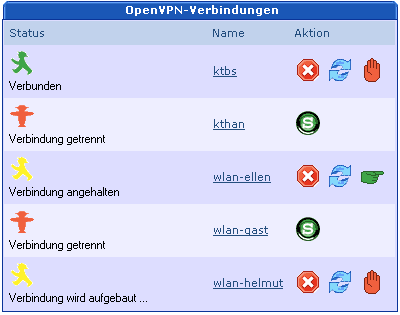
\includegraphics[width=400pt]{verbindungen}
    \caption{Aperçut des connexions}
    \label{fig:guiact}
  \end{figure}

\begin{description}
\item [Statut:] Le statut d'une liaison est symbolisé par un signal pour piéton.
  Lorsque le piéton est rouge cela signifie que le processus OpenVPN ne fonctionne
  pas, le piéton jaune que le processus ne fonctionne pas (encore) avec le poste
  éloigné, mais que la liaison peut être activée à tout moment et le piéton vert
  que la liaison est \flqq{}établie\frqq{}. Des informations plus précises sont
  indiquées en dessous des icônes piétons. Cela peut être instructif en
  particulier, pour le statut du piéton \flqq{}jaune\frqq{}.

\item [Nom:] Dans cette colonne, les noms des liaisons OpenVPN sont indiqués comme
  dans la configuration. En cliquant sur le nom, cela vous conduit dans une
  vue d'ensemble, dans laquelle est indiquée des informations plus précises de
  la liaison.

\item [Action:] Ici, les actions sont symbolisées par des icônes. Que signifie
  chaque icône? Voici ci-dessous un tableau récapitulatif~:

  \begin{table}[!h]
    \begin{tabular}{lp{12cm}}
      Symbole                                        & Explication \\
      \hline                                                            \\
      
\includegraphics[width=24pt]{start}            & Démarrer le processus OpenVPN et tente de se connecter. \\
      
\includegraphics[width=24pt]{stop}             & Arrête le processus OpenVPN. \\
      
\includegraphics[width=24pt]{reload}           & Réinitialise la connexion. \\
      
\includegraphics[width=24pt]{hold}             & stoppe la connexion, elle est en attente. Plus aucune donnée ne circule sur la liaison. \\
      
\includegraphics[width=24pt]{release}          & Relance la connexion. Les données peuvent à nouveau circuler sur la liaison. \\
      \hline                                                            \\
    \end{tabular}
  \caption{Commande du Webgui OpenVPN}
\end{table}
\end{description}

\subsubsection{OpenVPN~- WebGUI~- Vue détaillée d'une connexion}
  \begin{figure}[!h]
    \centering
    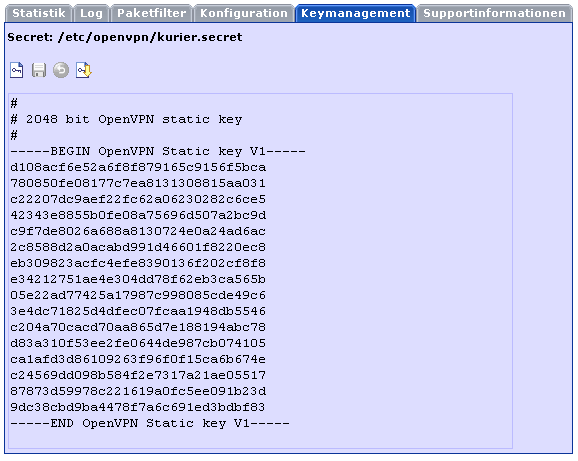
\includegraphics[width=400pt]{detail}
    \caption{Vue détaillée d'une connexion (gestion de clé)}
    \label{fig:guidetail}
  \end{figure}

\begin{description}
\item [Statistique:] on peut voir sur cet onglet, les statistiques
    intéressantes de la liaison. Les statistiques ne peuvent être visibles
    que si la liaison est démarrée et non arrêtée.

\item [Log:] On peut voir sur cet onglet, les 20 dernières lignes de la
    connexion. Si vous voulez voir plus de lignes, vous pouvez indiquer
    le nombre et cliquer sur "afficher". Si vous indiquez "all" vous
    pouvez voir la totalité du fichier log. Cet onglet est visible que
    si la liaison est démarrée.

\item [Debug-Log:] on peut voir sur cet onglet le processus de démarrage.
    On voit le démarrage de la liaison OpenVPN et ces sorties. C'est
    utile lorsque que l'on veut démarrer la liaison avec l'icône démarrée
    et que la connexion ne veut pas s'activer, en plus dans le fichier log
    normal il n'y a rien d'indiqué sur le démarrage.

\item [Filtrage de paquets:] on peut voir sur cet onglet le filtrage de paquets
    valide pour une liaison. Le filtrage de paquets est configuré que si
    la liaison est démarrée et que le tunnel est installé.

\item [Bridge:] on peut voir sur cet onglet la configuration du Bridge sur
    le routeur. Cet onglet est visible que si la liaison avec Bridge est
    installée.

\item [Configuration:] on peut voir sur cet onglet, la configuration de la
    liaison générée par le boot.

\item [Gestion de clé:] sur cet onglet, on peut produire une clé pour une
    liaison et peut également être téléchargés, (voir l'illustration
    \ref{fig:guidetail}). Aucune clé n'existe (au premier démarrage) du VPN,
    vous devez la produire automatiquement. Il peut être transféré directement
    avec le Symbole Download ou être copier/coller dans un fichier texte.
    Cliquez sur l'icône disquette pour enregistrer la clé qui a été nouvellement
    produite sur le routeur, ce processus peut-être annulé, par un clic sur
    l'icône restauration.

\item [Support informations:] sont indiquées dans cet onglet, toutes les
    informations qui pourraient être pertinentes, si vous avez un problème. Vous
    pouvez transmettre ces renseignements, par exemple pour un article
    dans des Newsgroups en faisant un copier/coller.

\end{description}


\subsection{OpenVPN~- Aide pour différentes versions OpenVPN }

Avec les versions différentes d'OpenVPN, vous devez veiller à l'utilisation
les paramètres, car les valeurs standards diffèrent pour chaque liaison VPN.
Cela concerne en particulier les réglages, MTU, FRAGMENT et MSSFIX. Si les
valeurs correspondent ne sont pas \flqq{}adaptées\frqq{} aux config OpenVPN
ou si la connexion fonctionne avec la commande ping, mais se bloque par exemple
lors de l'utilisation ssh, alors ces valeurs ne sont peut être pas ajustées
correctement. Voici les messages d'erreurs typiques, pour de tels cas~:

\begin{example}
\begin{verbatim}
FRAG_IN error flags=0xfa2a187b: FRAG_TEST not implemented
FRAG_IN error flags=0xfa287f34: spurrious FRAG_WHOLE flags
\end{verbatim}
\end{example}

Les paramètres cruciaux, pour la réalisation d'une liaison sont les suivants~:

\begin{description}

\item [OPENVPN\_x\_TUN\_MTU] La valeur MTU du périphérique TUN est pour 
  la version OpenVPN 1.x à 1300. La valeur à partir de la version OpenVPN 2.0
  est de 1500, valeur standard. 

\item [OPENVPN\_x\_LINK\_MTU] Taille en octet de la liaison des deux démons
  OpenVPN. Cette valeur par défaut est fonction de l'utilisation de la version
  OpenVPN et du système d'exploitation.

\item [OPENVPN\_x\_FRAGMENT] Les paquets (peu importe que ce soit UDP ou TCP)
  dont la taille est au-dessus du seuil de fragmentation, ces paquets de données
  seront fragmentés, et ne seront pas supérieures à celles indiquées dans la
  variable \var{OPENVPN\_x\_FRAGMENT} en octet.

\item [OPENVPN\_x\_MSSFIX] Afin d'échangent les paquets de données TCP sur une
  liaison VPN, sans que ces paquets soit si possible fragmentés, vous pouvez
  indiquer ici la dimension maximale souhaitée des paquets donnés TCP. Les
  systèmes d'exploitation actuels analysent mieux les normes de fragmentation,
  ainsi la fragmentation des paquets de données n'est plus nécessaire.

\end{description}

Les différentes versions OpenVPN utilisent les valeurs suivantes en tant que
valeurs par défaut. Vous devez faire attention à ces valeurs, si vous voulez
connecter ces versions OpenVPN qui ne fonctionnent pas sur le routeur fli4l.
Les valeurs par défaut spécifiées sur le routeur fli4l sont dans le deuxième
tableau.

\begin{table}[htbp]
  \begin{scriptsize}
    \begin{tabular}{lll}
       Option/version OpenVPN       & 1.xx                & 2.00        \\
      \hline                                                    \\
      OPENVPN\_x\_TUN\_MTU          & 1300                & 1500        \\
      OPENVPN\_x\_TUN\_MTU\_EXTRA   & inconnu             & 32          \\
      OPENVPN\_x\_FRAGMENT          & inconnu             & non configuré  \\
      OPENVPN\_x\_MSSFIX            & non configuré       & 1450        \\
    \end{tabular}
  \end{scriptsize}
  \caption{Paramètre MTU des différentes versions OpenVPN.}
\end{table}

\begin{table}[htbp]
  \begin{scriptsize}
    \begin{tabular}{lll}
     Option/version fli4l          & jusqu'à 2.1.8  & à partir  2.1.9  \\
      \hline                                                    \\
      OPENVPN\_x\_TUN\_MTU          & 1300                & 1500        \\
      OPENVPN\_x\_TUN\_MTU\_EXTRA   & 64                  & 32          \\
      OPENVPN\_x\_FRAGMENT          & non configuré       & 1300        \\
      OPENVPN\_x\_MSSFIX            & non configuré       & 1300        \\
    \end{tabular}
  \end{scriptsize}
  \caption{Paramètre MTU des différentes versions pour le routeur fli4l.}
\end{table}

En raison de ces différents paramètres, vous devez déterminer les valeurs par
défaut à installer dans votre réseau et écrire alors explicitement ceux-ci
dans le fichier config/openvpn.txt. Les valeurs sont dans la plupart des cas,
des valeurs satisfaisantes pour des premiers tests.

\begin{example}
\begin{verbatim}
OPENVPN_DEFAULT_TUN_MTU='1500'
OPENVPN_DEFAULT_MSSFIX='1300'
OPENVPN_DEFAULT_FRAGMENT='1300'
\end{verbatim}
\end{example}

Malheureusement, il n'est pas possible pour les versions fli4l antérieures à 2.1.9
de paramétrer directement le \flqq{}tun-mtu\frqq{}. Toutefois, on peut influencer
indirectement sur ce paramètre avec la variable \var{OPENVPN\_x\_LINK\_MTU}. La valeur
tun-mtu est d'environ 45 octets inférieurs à la valeur spécifiée dans
\var{OPENVPN\_x\_LINK\_MTU}. Pour déterminer la valeur précise, vous devez faire des essais.


\subsection{OpenVPN~- Exemples}

Quelques exemples illustrent la configuration du paquetage OpenVPN.

\subsubsection{Exemple~- Joindre deux réseaux par le routeur fli4l}

Dans le premier exemple, nous allons effectuer une liaison OpenVPN sur deux
routeurs fli4l. Il s'agit d'accéder au réseau derrière le routeur fli4l du poste
distant. Dans cet exemple, Peter et Maria veulent relier leurs réseaux par leur
routeur fli4l. Peter utilise l'adresse 192.168.145.0/24 pour le réseau privés
et l'adresses peter.eisfair.net pour DynDNS. Maria, utilise de façon
semblable l'adresse 10.23.17.0/24 pour le réseau et l'adresse maria.eisfair.net
pour DynDNS. Les deux se font confiance mutuellement et pourrons avoir accès à
l'ensemble de leurs réseaux.

\begin{table}[htbp]
  \begin{scriptsize}
    \begin{tabular}{lll}
      Option OpenVPN                 & Peter               & Maria               \\
      \hline \\
      OPENVPN\_1\_NAME=              & 'maria'             & 'peter'             \\
      OPENVPN\_1\_REMOTE\_HOST=      & 'maria.eisfair.net' & 'peter.eisfair.net' \\
      OPENVPN\_1\_REMOTE\_PORT=      & '10000'             & '10001'             \\
      OPENVPN\_1\_LOCAL\_PORT=       & '10001'             & '10000'             \\
      OPENVPN\_1\_SECRET=            & 'pema.secret'       & 'pema.secret'       \\
      OPENVPN\_1\_TYPE=              & 'tunnel'            & 'tunnel'            \\
      OPENVPN\_1\_REMOTE\_VPN\_IP=   & '192.168.200.202'   & '192.168.200.193'   \\
      OPENVPN\_1\_LOCAL\_VPN\_IP=    & '192.168.200.193'   & '192.168.200.202'   \\
      OPENVPN\_1\_ROUTE\_N=          & '1'                 & '1'                 \\
      OPENVPN\_1\_ROUTE\_1=          & '10.23.17.0/24'     & '192.168.145.0/24'  \\
      OPENVPN\_1\_PF\_INPUT\_N=      & '1'                 & '1'                 \\
      OPENVPN\_1\_PF\_INPUT\_1=      & 'ACCEPT'            & 'ACCEPT'            \\
      OPENVPN\_1\_PF\_FORWARD\_N=    & '1'                 & '1'                 \\
      OPENVPN\_1\_PF\_FORWARD\_1=    & 'ACCEPT'            & 'ACCEPT'            \\
    \end{tabular}
  \end{scriptsize}
  \caption{Configuration d'OpenVPN avec 2 routeurs fli4l}
\end{table}

\subsubsection{Exemple~- Deux réseaux reliés par un Bridge (ou pont)}

Dans l'exemple suivant, un Bridge est développé par l'intermédiaire une
connexion sans fil. Avec un Bridge, le filtrage de paquets ne peut pas être
configuré judicieusement, puisque seuls les frames Ethernet sont transmises,
absolument pas les paquets IP. Merci de ne pas oublier, qu'un réseau commun
doit être utiliser dans une configuration de bridge. En plus, il ne faut pas
que l'adresse IP soit attribuée deux fois.

\begin{table}[htbp]
  \begin{scriptsize}
    \begin{tabular}{lll}
      Option OpenVPN           & Peter          & Maria            \\
      \hline \\
      OPENVPN\_2\_NAME         & 'bridge'        & 'bridge'        \\
      OPENVPN\_2\_REMOTE\_HOST & '10.1.0.1'      & '10.2.0.1'      \\
      OPENVPN\_2\_REMOTE\_PORT & '10005'         & '10006'         \\
      OPENVPN\_2\_LOCAL\_HOST  & '10.2.0.1'      & '10.1.0.1'      \\
      OPENVPN\_2\_LOCAL\_PORT  & '10006'         & '10005'         \\
      OPENVPN\_2\_FLOAT        & 'no'            & 'no'            \\
      OPENVPN\_2\_RESTART      & 'never'         & 'never'         \\
      OPENVPN\_2\_SECRET       & 'bridge.secret' & 'bridge.secret' \\
      OPENVPN\_2\_TYPE         & 'bridge'        & 'bridge'        \\
      OPENVPN\_2\_BRIDGE       & 'pema-br'       & 'pema-br'       \\
    \end{tabular}
  \end{scriptsize}
  \caption{Configuration d'OpenVPN avec 2 routeurs fli4l leurs réseaux ont une connexion sans fil et utilise un Bridge}
\end{table}

Naturellement En plus des paramètres d'OpenVPN, vous devez configurer le Bridge
dans advanced\_networking et aussi de configurer base.txt, de telle sorte que
le Bridge soit utilisé en tant que périphérique réseau et non pas eth0 pour le
réseau interne. Ci-dessous nous avons adapté la configuration de
advanced\_networking et de base.

\begin{table}[htbp]
  \begin{scriptsize}
    \begin{tabular}{lll}
     Option advanced\_networking   & Peter           & Maria       \\
      \hline \\
      OPT\_BRIDGE\_DEV             & 'yes'           & 'yes'       \\
      BRIDGE\_DEV\_BOOTDELAY       & 'no'            & 'no'        \\
      BRIDGE\_DEV\_N               & '1'             & '1'         \\
      BRIDGE\_DEV\_1\_NAME         & 'pema-br'       & 'pema-br'   \\
      BRIDGE\_DEV\_1\_DEVNAME      & 'br0'           & 'br0'       \\
      BRIDGE\_DEV\_1\_DEV\_N       & '1'             & '1'         \\
      BRIDGE\_DEV\_1\_DEV\_1\_DEV  & 'eth0'          & 'eth0'      \\
    \end{tabular}
  \end{scriptsize}
  \caption{Configuration d'OpenVPN avec 2 routeurs fli4l leurs réseaux ont une connexion sans fil et utilise un Bridge, configuration dans advanced\_networking.}
\end{table}

\begin{table}[htbp]
  \begin{scriptsize}
    \begin{tabular}{lll}
     Option base            & Peter                 & Maria                \\
      \hline \\
      IP\_NET\_N            & '1'                   & '1'                  \\
      IP\_NET\_1            & '192.168.193.254/24'  & '192.168.193.1/24'   \\
      IP\_NET\_1\_DEV       & 'br0'                 & 'br0'                \\
    \end{tabular}
  \end{scriptsize}
  \caption{Configuration d'OpenVPN avec 2 routeurs fli4l leurs réseaux ont une connexion sans fil et utilise un Bridge, configuration dans (base.txt).}
\end{table}

\subsubsection{Exemple~- Configuration pour un accès Road warrior (ou Guerre commerciale informatisée)}

\marklabel{roadwarrior} Pour cet exemple (Road warrior), un portable sous Windows
XP est permis et un accès GPRS pour accéder au RÉSEAU LOCAL derrière le routeur fli4l.
Sur le portable est installé un OpenVPN pour Windows XP, le fichier *.ovpn
correspondant doit être adapté. Malheureusement, les pilotes tun/tap sous Windows
ne sont pas aussi souples que son homologue Unix. C'est pourquoi avec le Point-to-Point
pour VPN les adresses IP doivent se trouver dans le réseau 255.255.255.252 (ou /30).
Si Road Warrior doit seulement accéder aux services du LAN derrière le
routeur fli4l, il ne sera pas nécessaire d'indiquer un itinéraire sur la page fli4l,
comme cela il ne réagira pas. Avec Road warrior si nécessaire on peut utiliser une
adresse IP virtuels dans (\var{OPENVPN\_3\_REMOTE\_VPN\_IP}). Si Road warrior
dispose d'une adresse IP statique, on pourra également enregistrer une route pour un hôte,
par ex. si Road warrior a une adresse IP 192.168.33.33 statique, vous pouvez insérer
dans le fichier de configuration openvpn.txt de fli4l~:

\begin{example}
\begin{verbatim}
OPENVPN_3_ROUTE_N='1'
OPENVPN_3_ROUTE_1='192.168.33.33/32'
\end{verbatim}
\end{example}

Au sujet de la configuration de filtrage de paquets ci-dessous, il vous permet
une communication complète dans les deux sens. Road warrior ne peut pas interroger
directement le routeur fli4l. Mais si c'est nécessaire, il est possible d'utilise
le serveur DNS du routeur fli4l.

\begin{example}
\begin{verbatim}
OPENVPN_3_PF_FORWARD_N='1'
OPENVPN_3_PF_FORWARD_1='ACCEPT'
\end{verbatim}
\end{example}

Si Road warrior est autorisé pour accéder au serveur DNS interne du routeur fli4l,
il faut ajouter dans la configuration de fli4l les paramètres suivant~:

\begin{example}
\begin{verbatim}
OPENVPN_3_PF_INPUT_N='1'
OPENVPN_3_PF_INPUT_1='if:VPNDEV:any tmpl:dns ACCEPT'
\end{verbatim}
\end{example}

\begin{table}[htbp]
  \begin{scriptsize}
    \begin{tabular}{ll}
      Option OpenVPN routeur fli4l                  & roadwarrior           \\
      \hline \\
      OPENVPN\_3\_NAME='roadwarrior'                & remote peter.eisfair.net \\
      OPENVPN\_3\_LOCAL\_PORT='10011'               & rport 10011 \\
      OPENVPN\_3\_SECRET='roadwarrior.secret'       & secret roadwarrior.secret \\
      OPENVPN\_3\_TYPE='tunnel'                     & dev tun \\
      OPENVPN\_3\_REMOTE\_VPN\_IP='192.168.200.238' & ~ \\
      OPENVPN\_3\_LOCAL\_VPN\_IP='192.168.200.237'  & ifconfig 192.168.200.238 192.168.200.237 \\
      OPENVPN\_3\_ROUTE\_N='0'                      & ~ \\
      OPENVPN\_3\_PF\_FORWARD\_N='1'                & ~ \\
      OPENVPN\_3\_PF\_FORWARD\_1='ACCEPT'           & ~ \\
      ~                                             & route 192.168.145.0 255.255.255.0 \\
      ~                                             & comp-lzo \\
      ~                                             & persist-tun \\
      ~                                             & persist-key \\
      ~                                             & ping-timer-rem \\
      ~                                             & ping-restart 60 \\
      ~                                             & proto udp4 \\
      ~                                             & tun-mtu 1500 \\
      ~                                             & fragment 1300 \\
      ~                                             & mssfix \\
    \end{tabular}
  \end{scriptsize}
  \caption{Configuration d'OpenVPN pour un ordinateur Windows avec GPRS}
\end{table}

\subsubsection{Exemple~- Liaison WLAN sécurisé}

Dans cet exemple, on passe par un WLAN (ou sans fil) pour accéder à la liaison
OpenVPN. On part du principe que le WLAN est installé sur le routeur fli4l , une
carte Ethernet pour le réseau local et une carte WLAN, dont le point d'accès est
activé. L'objectif doit être, un Client WLAN sans liaison VPN a seulement accès
au VPN par le port du routeur fli4l. Ce n'est qu'après la connexion réussite
avec OpenVPN, que l'échange sans restriction avec le réseau local du poste
distant peut être possible. Pour cela des modifications du serveur DNSMASQ
DHCP doivent être réalisées. En outre, le paquetage advanced\_networking est
nécessaire à l'installation. Il faut aussi paramétrer \var{IP\_NET\_1} pour
le LAN (réseau local) et \var{IP\_NET\_2} pour le WLAN (réseau sans fil) dans
le fichier base.txt.

\begin{example}
\begin{verbatim}
IP_NET_N='2'
IP_NET_1='192.168.3.254/24'
IP_NET_1_DEV='br0'
IP_NET_2='192.168.4.254/24'
IP_NET_2_DEV='eth2'
\end{verbatim}
\end{example}

La plage DHCP doit être réglé selon vos besoins. Pour la variable \var{IP\_NET\_2}
vous devez absolument ajouter les paramètres suivants~:

\begin{example}
\begin{verbatim}
DNSDHCP_RANGE_2_DNS_SERVER1='none'
DNSDHCP_RANGE_2_NTP_SERVER='none'
DNSDHCP_RANGE_2_GATEWAY='none' 
\end{verbatim}
\end{example}

Paramètre advanced\_networking.txt~:
 
\begin{example}
\begin{verbatim}
OPT_BRIDGE_DEV='yes'
BRIDGE_DEV_BOOTDELAY='yes'
BRIDGE_DEV_N='1'
BRIDGE_DEV_1_NAME='br'
BRIDGE_DEV_1_DEVNAME='br0'
BRIDGE_DEV_1_DEV_N='1'
BRIDGE_DEV_1_DEV_1_DEV='eth0'
\end{verbatim}
\end{example}

\begin{table}[htbp]
  \begin{scriptsize}
    \begin{tabular}{ll}
      Option OpenVPN routeur                        & Client WLAN\\
      \hline \\
      OPENVPN\_4\_NAME='wlan1'                      & ~ \\
      OPENVPN\_4\_LOCAL\_HOST='192.168.4.254'       & remote 192.168.4.254\\
      OPENVPN\_4\_LOCAL\_PORT='20001'               & rport 20001 \\
      OPENVPN\_4\_SECRET='wlan1.secret'             & secret wlan1.secret \\
      OPENVPN\_4\_TYPE='bridge'                     & dev tap\\
      OPENVPN\_4\_BRIDGE='br'                       & ~\\
      OPENVPN\_4\_RESTART='never'                   & ~\\
      OPENVPN\_4\_MUTE\_REPLAY\_WARNINGS='yes'      & ~\\
      ~                                             & comp-lzo \\
      ~                                             & persist-tun \\
      ~                                             & persist-key \\
      ~                                             & ping-timer-rem \\
      ~                                             & ping-restart 60 \\
      ~                                             & proto udp4 \\
      ~                                             & tun-mtu 1500 \\
      ~                                             & fragment 1300 \\
      ~                                             & mssfix \\
    \end{tabular}
  \end{scriptsize}
  \caption{OpenVPN sécurisé dans un WLAN}
\end{table}


\subsection{Liens sur le thème OpenVPN}

Pour terminer, encore quelques liens qui traitent de la configuration OpenVPN~:

\noindent \altlink{http://openvpn.net} \\
\altlink{http://de.wikipedia.org/wiki/OpenVPN} \\
\altlink{http://openvpn.se/} \\
% \altlink{http://www.vpnforum.de/} \\
\altlink{http://arnowelzel.de/wiki/en/fli4l/openvpn} \\
\altlink{http://wiki.freifunk.net/OpenVPN} \\
\altlink{http://w3.linux-magazine.com/issue/24/Charly.pdf} \\
\altlink{http://w3.linux-magazine.com/issue/25/WirelessLAN_Intro.pdf} \\
\altlink{http://w3.linux-magazine.com/issue/25/OpenVPN.pdf} \\
% \altlink{http://www.0dx.de/linux/linuxmag/1994_2009/2002/08/sysadauf/sysadauf.html} \\
% \altlink{http://bilbo.naumann-net.org/~ms/aklininst/folien/01/openvpn.pdf} \\
% \altlink{http://lists.spline.inf.fu-berlin.de/pipermail/fli4l_dev/2005-May/016101.html} \\

\appendix
  \chapter{Anhang zum Paket OPENVPN}
  \input{openvpn_appendix}
  \listoffigures
  \listoftables
  \printindex


\end{document}

